\chapter{Conceptos Preliminares}

    %\thispagestyle{empty}

    \lettrine[lines=5] { \initfamily \selectfont E}{s} imposible estudiar una teoría matemática sin antes establecer sus definiciones básicas y su notación respectiva. En este capítulo desglosaremos brevemente las ideas y la terminología de las dos ramas de las Matemáticas involucradas en esta tesis. Muchos de los resultados mencionados aquí los dejaremos sin demostración ya que no es nuestro objetivo principal.
    
 

    \section{Álgebra Lineal}
        A continuación abordaremos los conceptos y las notaciones de las que haremos uso a lo largo de este trabajo. Si el lector está interesado en profundizar en estos temas, y desea conocer las demostraciones de los teoremas mencionados, se le invita a revisar \cite{Friedberg,Noble,Zhang, Shores}.

        \subsection{¿Qué es un espacio vectorial?}
            Un \textit{campo}\index{Campo} $\mathbb{F}$ es un conjunto, en el cual están definidas dos operaciones \\ $+$ y $\bullet$, llamadas \textit{suma} y \textit{multiplicación}, respectivamente, de tal manera que por cada par de elementos $x,y \in \mathbb{F}$, existen únicos $x+y$ y $x \bullet y$ en $\mathbb{F}$. Además, para todo $a,b,c \in \mathbb{F}$, deben cumplirse las siguientes condiciones\index{Campo! propiedades de}: 
                \begin{enumerate}
                    \item \textit{Conmutatividad de la suma y multiplicación}:
                        $a + b = b + a$  y  $a \bullet b = b \bullet a$
                    \item \textit{Asociatividad de la suma y multiplicación}:
                        $(a + b) + c = a + (b + c)$  y  $(a \bullet b)\bullet c = a\bullet(b \bullet c)$.
                    \item \textit{Existencia del neutro aditivo y del neutro multiplicativo}:
    
                        Existen  $0, 1 \in\mathbb{F}$, tales que:
                         $0 + a = a$  y  $1 \bullet a = a$.
    
                    \item \textit{Existencia del inverso aditivo y del inverso multiplicativo}:
    
                        Para cualesquiera $a$ en $\mathbb{F}$ y  $b \neq 0$ en $\mathbb{F}$, existen $c$ y $d$ en $\mathbb{F}$ tales que:
                        $a + c  =  0$  y  $b \bullet d  =  1$.
                        
                    \item \textit{Distributividad de la multiplicación sobre la suma}:
                        $a \bullet(b + c)  = a \bullet b  +  a \bullet c$
                 \end{enumerate}

            El campo más sencillo con el que trabajaremos en esta tesis es el campo de Galois\footnote{Otros autores lo denotan como $\mathbb{Z}_{2}$ o $\mathbb{F}_{2}$.} $GF(2)$. Este campo es el conjunto $\{0,1\}$ con las operaciones dadas por las siguientes tablas:

            \begin{center}
                \begin{tabular}{ c | c c }
                    + & 0 & 1 \\ \hline
                    0 & 0 & 1 \\  
                    1 & 0 & 0    
                \end{tabular}
            \end{center}

            \begin{center}
                \begin{tabular}{ c | c c }
                    $\bullet$ & 0 & 1 \\ \hline
                    0 & 0 & 0 \\  
                    1 & 0 & 1    
                \end{tabular}
            \end{center}

            Puede notarse que la suma en $GF(2)$ coincide con el álgebra módulo $2$ en los números enteros.

            Otros campos más utilizados son los números reales $\mathbb{R}$ y los complejos $\mathbb{C}$ con la suma y multiplicación usuales.


            Un \textit{espacio vectorial $V$ sobre un campo $\mathbb{F}$}\index{Espacio! vectorial} consiste de un conjunto $V$ con dos operaciones definidas en él, llamadas  \textit{suma} $+$ y \textit{multiplicación \\ escalar} $\cdot$, tales que, para cualesquiera $\mathbf{x,y} \in V$ y todo $k \in \mathbb{F}$, existen únicos $\mathbf{x + y} \in V$ y $k \cdot \mathbf{x} \in V$. Además, estas operaciones deben cumplir lo siguiente:
 
            \begin{enumerate}
                \item Para cualesquiera $\mathbf{x,y} \in V$, $\mathbf{x + y = y + x}$.
                \item Para cualesquiera $\mathbf{x,y,z} \in V$, $\mathbf{(x+y)+z = x+ (y+z)}$.
                \item Existe un elemento $\mathbf{0} \in V$ tal que, para todo $\mathbf{x} \in V$, $\mathbf{x + 0 = x}$.
                \item Para todo $\mathbf{x} \in V$, existe $\mathbf{-x} \in V$ tal que $\mathbf{x + (-x) = 0}$.
                \item Para todo $\mathbf{x}$, $1 \cdot \mathbf{x} = \mathbf{x}$.
                \item Para cualesquiera $a,b \in \mathbb{F}$, y todo $\mathbf{x} \in V$, $(ab)\cdot \mathbf{x} = a(b\cdot\mathbf{x})$.
                \item Para todo $a \in \mathbb{F}$, y cualesquiera $\mathbf{x,y}$, $a \cdot (\mathbf{x + y}) = a\cdot \mathbf{x} + a\cdot \mathbf{y}$.
                \item Para cualesquiera $a,b \in \mathbb{F}$, y todo $\mathbf{x}$, $(a+b) \cdot (\mathbf{x}) = a\cdot \mathbf{x} + b\cdot \mathbf{x}$.
            \end{enumerate}
 
            A los elementos de $\mathbb{F}$ les llamamos \textit{escalares}\index{Escalar} y los de $V$ los nombramos \textit{vectores}\index{Vector}. Una $n-$ada ordenada es un vector del espacio $\mathbb{F}^{n}$, y la escribimos en \textit{forma de columna}. Así, dados $a_{1}, \ldots, a_{n} \in \mathbb{F}$, escribimos 
                $$
                \begin{bmatrix}
                    a_{1} \\
                    \vdots \\
                    a_{n}
                \end{bmatrix} \in \mathbb{F}^{n}.
                $$

            Dependiendo de la situación, estas $n-$adas se escribirán en \textit{forma de renglón} agregando un superíndice ``$\mathbf{t}$'', es decir:
                $$
                \begin{bmatrix}
                    a_{1} & \cdots & a_{n}
                \end{bmatrix} ^{\mathbf{t}} \in \mathbb{F}^{n}.
                $$

            Resulta que $\mathbb{F}^{n}$ es uno de los espacios vectoriales más conocidos, cuya suma y producto escalar se hacen \textit{entrada a entrada} con la suma y producto del campo $\mathbb{F}$. En efecto, sean $\begin{bmatrix} a_{1} & \cdots & a_{n}\end{bmatrix} ^{\mathbf{t}}, \begin{bmatrix} b_{1} & \cdots & b_{n} \end{bmatrix} ^{\mathbf{t}} \in \mathbb{F}^{n}$ y $k \in \mathbb{F}$. Entonces
                $$
                \begin{bmatrix}
                a_{1} \\
                \vdots \\
                a_{n}
                \end{bmatrix} + \begin{bmatrix}
                b_{1} \\
                \vdots \\
                b_{n}
                \end{bmatrix}  =\begin{bmatrix}
                a_{1} + b_{1} \\
                \vdots \\
                a_{n} + b_{n}
                \end{bmatrix} \in \mathbb{F}^{n}
                $$ y $$ k \cdot\begin{bmatrix}
                a_{1} \\
                \vdots \\
                a_{n}
                \end{bmatrix} = \begin{bmatrix}
                ka_{1} \\
                \vdots \\
                ka_{n}
                \end{bmatrix} \in \mathbb{F}^{n}.$$

            Por supuesto, $\mathbb{R}^{n}$ y $\mathbb{C}^{n}$ son espacios vectoriales. Si $\mathbb{F} = GF(2)$, entonces denotamos por $\oplus$ a la suma en $GF(2)^{n}$. Ésta, desde luego, se hace entrada a entrada siguiendo las operaciones que exhibimos en tablas líneas arriba. Por ejemplo, tomemos $\begin{bmatrix} 1 & 0 & 1 & 1 \end{bmatrix}^{\mathbf{t}}$ y $\begin{bmatrix} 0 & 1 & 1 & 1 \end{bmatrix}^\mathbf{t}$ en $GF(2)^{4}$. Entonces 
                $$ \begin{bmatrix}
                1 \\
                0 \\
                1\\
                1
                \end{bmatrix} \oplus \begin{bmatrix}
                0 \\
                1\\
                1\\
                1
                \end{bmatrix}  =\begin{bmatrix}
                1 \\
                1 \\
                0\\
                0
                \end{bmatrix}.
                $$

            Un subconjunto $W$ de un espacio vectorial $V$ sobre $\mathbb{F}$ es un \textit{subespacio vectorial} si $W$ es un espacio vectorial sobre $\mathbb{F}$ con las mismas operaciones definidas en $V$. De hecho, se sabe que $W$ es un subespacio si  y sólo si $\mathbf{0} \in W$, $\mathbf{x + y} \in W$, para cualesquiera $\mathbf{x,y} \in W$; y $k\mathbf{x} \in W$, para todo $k \in \mathbb{F}$ y $\mathbf{x} \in W$.

        \subsection{Combinaciones lineales e independencia lineal}
            Dado un  espacio vectorial $V$ y $S \subseteq V$, decimos que $\mathbf{v} \in V$ es una \textit{combinación lineal de vectores de $S$} si existe una cantidad finita de vectores $\mathbf{u_{1}, \ldots, u_{n}} \in S$ y escalares $k_{1}, \ldots, k_{n}\in \mathbb{F}$ tales que $\mathbf{v} = k_{1}\mathbf{u}_{1} + \cdots + k_{n}\mathbf{u}_{n}$. Usualmente llamamos \textit{coeficientes} a los escalares de la combinación lineal.

            El conjunto de todas las posibles combinaciones lineales de vectores en $S$ es llamado el \textit{generado de $S$} y lo escribimos $span(S)$. Este conjunto es un subespacio de $V$. Si $span(S) = V$, se dice que $S$ \textit{genera} a $V$.

            Si hacemos una combinación lineal $k_{1}\mathbf{u}_{1} + \cdots +k_{n}\mathbf{u}_{n} = \mathbf{0} $, con \\ $k_{1} = \ldots= k_{n} = 0$, ésta es llamada una \textit{combinación lineal trivial} del $\mathbf{0}$. Un conjunto de vectores $S$ se dice que es \textit{linealmente dependiente} si existe una combinación lineal del $\mathbf{0}$ no trivial con vectores de $S$. En caso contrario, esto es, cuando la única combinación lineal del $\mathbf{0}$ es la trivial, se dice que $S$ es un conjunto \textit{linealmente independiente}.

            Se sabe que si $S \subseteq T$ y $T$ es linealmente independiente, entonces $S$ es también linealmente independiente. Si $S$ es linealmente dependiente, necesariamente $T$ también lo es. También se conoce que, si $\mathbf{u} \notin S$, entonces $S\cup \{\mathbf{u}\}$ es linealmente dependiente si y sólo si $\mathbf{u} \in span(S)$.

            Una \textit{base} de $V$ es un subconjunto linealmente independiente $\beta$ de $V$ tal que $span(\beta) = V$. Las bases de los espacio vectoriales resultan ser de suma importancia. Por ejemplo, todo vector puede expresarse de manera única como combinación lineal de vectores de $\beta$.

            Cualquier base de un espacio vectorial tiene la misma cantidad de vectores. Este número de vectores en cualquier base se le conoce como la \textit{dimensión} del espacio vectorial y se le denota como $\dim(V)$. Todos los espacios con los que trabajaremos aquí son de \textit{dimensión finita}.


            Una base para $\mathbb{F}^{n}$ es aquella conformada por los vectores canónicos $\mathbf{e}_{i}$ cuya $i-$ésima entrada es $1$ y $0$ en las demás. Así, $\dim(\mathbb{F}^{n}) = n$.

            Se sabe que la cantidad de elementos en un conjunto linealmente independiente no puede exceder la dimensión del espacio. La cantidad de elementos en un conjunto generador no puede ser menor que dicha dimensión. En otras palabras, si $S$ es linealmente independiente en $V$ y $span(T)=V$, entonces $|S| \leq \dim(V) \leq |T|$. También, si $W \subseteq V$ es un subespacio, entonces $\dim(W) \leq \dim(V)$.

            Dados $A,B \subseteq V$, definimos la suma de $A$ y $B$ como el conjunto $A+B := \{ \mathbf{x + y} \in V\ | \mathbf{x}\in A, \mathbf{y} \in B \}$ y resulta ser un subespacio de $V$.

            Dados dos subespacios $W_{1},W_{2} \subseteq V$, decimos que $V$ es suma directa de $W_{1}$ y $W_{2}$ si y sólo si $W_{1} \cap W_{2} = \{\mathbf{0}\}$ y $W_{1} + W_{2} = V$. En tal caso, escribimos $V = W_{1} \oplus W_{2}$. Es muy conocido que $\dim(V) = \dim(W_{1}) + \dim(W_{2})$. Incluso, si $\beta_{1}$ y $\beta_{2}$ son bases de $W_{1}$ y $W_{2}$, respectivamente, entonces $\beta_{1} \cup \beta_{2}$  es una base de $V$. Como es de suponerse, esta definición y estas afirmaciones se extienden para cualquier cantidad de subespacios vectoriales. 
            %\vspace{-0.15cm}
        \subsection{Transformaciones lineales}
            Las transformaciones lineales entre espacios vectoriales son una clase especial de funciones que preservan la estructura de los espacios. En \cite{Friedberg} hay un estudio extenso sobre ellas. Formalmente, sí $V$ y $W$ son espacios vectoriales (ambos  sobre $\mathbb{F}$), una función $T : V \rightarrow W$ es una \textit{transformación lineal} si para cualesquiera $\mathbf{x,y} \in V$ y todo $ c \in \mathbb{F}$, se cumple: $T(\mathbf{x + y}) = T(\mathbf{x}) + T(\mathbf{y})$ y $T(c\mathbf{x}) = cT(\mathbf{x})$.


            Hay dos subespacios vectoriales asociados a una transformación $T$. El \textit{Kernel} (o \textit{núcleo}) de $T$ es el conjunto $Ker(T):= \{ \mathbf{x} \in V | T(\mathbf{x}) = \mathbf{0}\}$. De igual manera, podemos hablar de la \textit{imagen} de $T$, que es el conjunto \\ $Im(T):= \{ T(\mathbf{x}) : \mathbf{x} \in V\}$.

            El \textit{rango} de $T$ es la dimensión de su imagen y la \textit{nulidad} de $T$ es la dimensión de su kernel, es decir,
                $$rank(T):= \dim(Im(T))\textnormal{ y } null(T):= \dim(Ker(T)).$$ 
            El famoso \textit{teorema de la dimensión} (o \textit{teorema de rango-nulidad}) establece que, si $V$ tiene dimensión finita, entonces $\dim(V)= rank(T) + null(T)$.

            Decimos que dos espacios $V$ y $W$ son \textit{isomorfos} si y sólo si existe una transformación lineal biyectiva $T \colon V \rightarrow W$. A tal transformación se le llama \textit{isomorfismo}.

            Muchas propiedades se derivan de aquí. Si dos espacios son isomorfos, entonces tienen la misma dimensión. Aún más, si $V$ es un espacio vectorial sobre $\mathbb{F}$ y $\dim(V) =n$, entonces $V$ es isomorfo a $\mathbb{F}^{n}$.


        \subsection{Ortogonalidad}
            Un espacio vectorial sobre el campo $\mathbb{F}=\mathbb{R}$ (ó $\mathbb{F}=\mathbb{C}$) es un \textit{espacio con producto interno} si está dotado de un \textit{producto interno} $\langle \cdot{,} \cdot \rangle$ que satisface, para todo $k \in \mathbb{F}$ y para cualesquiera $\mathbf{u,v,w} \in V$, lo siguiente:
                \begin{enumerate}
                    \item $\langle \mathbf{u,u}\rangle \geq 0$ y $\langle \mathbf{u,u}\rangle = 0$ si y sólo si $\mathbf{u} = \mathbf{0}$.
                    \item $\langle \mathbf{u+v,w} \rangle = \langle \mathbf{u,w} \rangle + \langle \mathbf{v,w}\rangle$.
                    \item $ \langle k\mathbf{u,v}\rangle =  k\langle \mathbf{u,v}\rangle$.
                    \item $\overline{ \langle \mathbf{u,v}\rangle} =  \langle \mathbf{v,u}\rangle$.
                \end{enumerate}

            Dados $\mathbf{x,y} \in \mathbb{R}^{n}$, el producto interno usual en $\mathbb{R}^{n}$ es $$ \langle \mathbf{x,y}\rangle = \sum_{i = 1}^{n} x_{i}y_{i}.$$
            Al tener un producto interno definido en $V$, obtenemos una noción de \textit{ortogonalidad} entre vectores. De hecho, se dice que dos vectores $\mathbf{x,y} \in V$ son ortogonales si y sólo si $ \langle \mathbf{x,y}\rangle =0$.

            Si $S$ es un subconjunto no vacío de $V$, entonces el \textit{complemento ortogonal} de $S$ es el conjunto $S^{\perp}$ de vectores ortogonales a todo vector de $S$, o sea, $$S^{\perp}:= \{\mathbf{x} \in V |  \langle \mathbf{x,y}\rangle = 0, \textnormal{para todo } y \in S\}.$$

            Puede demostrarse que $S^{\perp}$ es un subespacio vectorial. Para espacios vectoriales sobre campos finitos, como $GF(2)$, también podemos considerar como producto interno el usual, es decir, para todo $\mathbf{x,y} \in \mathbb{F}^{n}$, $ \langle \mathbf{x,y}\rangle =  \sum_{i = 1}^{n} x_{i}y_{i}$. No obstante, estos espacios vectoriales fallan en el primer punto de la definición, es decir, hay vectores $\mathbf{u}$ tales que $\langle \mathbf{u,u}\rangle = 0$ pero $\mathbf{u}\neq \mathbf{0}$. Tenemos, pues, que hay vectores \textit{ortogonales a sí mismos}. Llamamos a estos productos \textit{productos internos degenerados}. 

        \subsection{Matrices}
            Una \textit{matriz} $\mathbf{A}$ \textit{de} $n \times m$ \textit{sobre un campo} $\mathbb{F}$ es un arreglo rectangular de  $m$ renglones y $n$ columnas. El conjunto de estas matrices se escribe como $\mathbb{M}_{n \times m}(\mathbf{F})$. Los vectores columna de $n$ entradas, en particular, se pueden considerar como matrices de tamaño $1 \times n$. Frecuentemente escribimos $\mathbf{A} = [a_{ij}]$ para denotar abreviadamente a la matriz $\mathbf{A}$ y sus entradas, es decir,
                $$
                \mathbf{A}:= \begin{bmatrix}
                a_{11} & \cdots & a_{1m}\\ 
                \vdots & \ddots &\vdots\\ 
                a_{n1} &\cdots  & a_{nm} 
                \end{bmatrix}
                $$

            La matriz cuyas entradas son todas $0$ se escribe $\mathbf{O}$.
            Definimos la suma de dos matrices del mismo tamaño, $\mathbf{A} = [a_{ij}]$ y $\mathbf{B} = [b_{ij}]$ como la matriz $\mathbf{A+B}: = [a_{ij} + b_{ij}]$.

            También definimos el producto de un vector renglón y un vector columna. Sean $\mathbf{a}^{\mathbf{t}}:=\begin{bmatrix}
            a_{1} & \cdots & a_{m}\\ 
            \end{bmatrix}^{\mathbf{t}}$ y $\mathbf{b}:=\begin{bmatrix}
            b_{1} \\ 
            \vdots\\
            b_{m}\\ 
            \end{bmatrix}$. Entonces $$\mathbf{a}^{\mathbf{t}}\mathbf{b} = \begin{bmatrix}
            a_{1} & \cdots & a_{m}\\ 
            \end{bmatrix}^{\mathbf{t}} \begin{bmatrix}
            b_{1} \\ 
            \vdots\\
            b_{m}\\ 
            \end{bmatrix}:= [a_{1}b_{1} + \cdots + a_{m}b_{m}].$$

            Cuando tratamos con matrices, es útil manipularlas por sus columnas o por su renglones. Supongamos que $\mathbf{A} \in \mathbb{M}_{n \times m}(\mathbb{F})$, es de la forma
            $$
            \mathbf{A}= \begin{bmatrix}
            a_{11} & \cdots & a_{1m}\\ 
            \vdots & \ddots &\vdots\\ 
            a_{n1} &\cdots  & a_{nm} 
            \end{bmatrix}
            $$

            Entonces definimos la $j-$ésima \textit{columna de}  $\mathbf{A}$ como el vector de tamaño $n \times 1$ $$\mathbf{c}_{j} := \begin{bmatrix}
            a_{1j} \\ 
            \vdots\\
            a_{nj}
            \end{bmatrix}
            $$
            
             Escribimos $\mathbf{A} = \begin{bmatrix}
            \mathbf{c}_{1} | & \cdots & |\mathbf{c}_{m}
            \end{bmatrix}.$
            
            Análogamente, el $i-$ésimo \textit{renglón} de $\mathbf{A}$ es el vector de tamaño $1 \times n$ $\mathbf{r}_{i}:= \begin{bmatrix}
            a_{i1} & \cdots & a_{im}
            \end{bmatrix}.$ Y escribimos: $$\mathbf{A} = \begin{bmatrix}
            \mathbf{r}_{1}\\
            \--\\
            \vdots \\
            \--\\
            \mathbf{r}_{n}
            \end{bmatrix}.$$ Démonos cuenta que $\mathbf{c}_{j} \in \mathbb{F}^{n}$ y $\mathbf{r}_{i} \in \mathbb{F}^{m}$.
            
            De esta manera, dadas $\mathbf{A} \in \mathbb{M}_{n \times m}(\mathbb{F})$ y $\mathbf{B} \in \mathbb{M}_{m \times q}(\mathbb{F})$, el \textit{producto de $\mathbf{A}$ y $\mathbf{B}$} es la matriz $\mathbf{AB} \in \mathbb{M}_{n \times q}(\mathbb{F})$ de la forma $$ \mathbf{AB}:= \begin{bmatrix}
            \mathbf{r}_{1_{\mathbf{A}}}\mathbf{c}_{1_\mathbf{B}} | \cdots | \mathbf{r}_{m_{\mathbf{A}}}\mathbf{c}_{m_{\mathbf{B}}}
            \end{bmatrix}, $$ donde $\mathbf{r}_{i_\mathbf{A}}$ es el $i-$ésimo renglón de $\mathbf{A}$ y $\mathbf{c}_{i_\mathbf{B}}$ es la $i-$ésima columna de $\mathbf{B}$.
            
            
            El producto de una matriz de tamaño $n \times m$ por un vector de tamaño $m \times 1$ nos arroja otro vector de tamaño $n \times 1$. Dicho de otro modo, dado  $$\mathbf{x} = \begin{bmatrix}
            x_{1} \\
            \vdots \\
            x_{m}
            \end{bmatrix} \in \mathbb{F}^{m},$$ el producto $\mathbf{Ax}$ está dado por $$ \mathbf{Ax} =  \begin{bmatrix}
            \mathbf{c}_{1} | & \cdots & |\mathbf{c}_{m}
            \end{bmatrix} \begin{bmatrix}
            x_{1} \\
            \vdots\\
            x_{m}
            \end{bmatrix} = x_{1}\mathbf{c}_{1} + \cdots + x_{m}\mathbf{c}_{m} \in \mathbb{F}^{n}.
            $$
            
            El espacio generado por las columnas de $\mathbf{A}$ lo denotamos como $\mathsf{C}(\mathbf{A})$; y al espacio generado por los renglones lo escribimos como $\mathsf{R}(\mathbf{A})$. Similarmente a las transformaciones lineales, las matrices también tienen un kernel. Definimos el \textit{kernel} (o \textit{espacio nulo}) de la matriz $\mathbf{A}$ como el conjunto $$Ker(\mathbf{A}) := \{\mathbf{x} \in \mathbb{F}^{m} | \mathbf{Ax} = \mathbf{0}\}.
            $$
            
            Estos espacios vectoriales nos permiten definir el rango y la nulidad de una matriz. En efecto, el \textit{rango} de $\mathbf{A}$ es $rank(\mathbf{A}):= \dim(\mathsf{C}(\mathbf{A}))$ y la \textit{nulidad} de $\mathbf{A}$ es $null(\mathbf{A}):= \dim(Ker(\mathbf{A}))$.
            
            Puede probarse que $rank(\mathbf{A})= \dim(\mathsf{C}(\mathbf{A})) = \dim(\mathsf{R}(\mathbf{A})))$. Entonces, dados los conocimientos de espacios vectoriales y sus dimensiones, suele decirse que el rango de una matriz es \textit{el máximo número de sus columnas linealmente independientes} o \textit{el máximo número de sus renglones linealmente independientes}. Otra propiedad importante es  que $(\mathsf{R}(\mathbf{A}))^{\perp} = Ker(\mathbf{A})$ y $(Ker(\mathbf{A}))^{\perp} = \mathsf{R}(\mathbf{A})$.
            
            Dadas dos matrices $\mathbf{A}$ y $\mathbf{B}$, si las columnas y renglones de $\mathbf{B}$ están contenidas en las columnas y renglones de $\mathbf{A}$, entonces decimos que $\mathbf{B}$ es \textit{submatriz} de $\mathbf{A}$. 
            
             Una matriz $\mathbf{A}$ puede \textit{partirse} en varias submatrices. Por ejemplo, $\mathbf{A}$ puede escribirse de la forma $$\mathbf{A} = \begin{bmatrix}
            \mathbf{B} & \mathbf{C} \\
            \mathbf{I} & \mathbf{O}
            \end{bmatrix}.$$ 
            
            En tal caso, se dice que $\mathbf{A}$ tiene una \textit{partición por} \textit{bloques}. Si partimos a $\mathbf{A}$ en submatrices $\mathbf{A}_{i}$ de manera que $$\mathbf{A} = \begin{bmatrix}
            \mathbf{A}_{1} & \cdots & \mathbf{O} \\
            \vdots & \ddots & \vdots \\
            \mathbf{O} & \cdots & \mathbf{A}_{c}
            \end{bmatrix},$$ podemos probar que $\mathsf{C}(\mathbf{A}) = \mathsf{C}(\mathbf{A}_{1})\oplus \cdots \oplus \mathsf{C}(\mathbf{A}_{c})$ y también \\ $\mathsf{R}(\mathbf{A}) = \mathsf{R}(\mathbf{A}_{1})\oplus \cdots \oplus \mathsf{R}(\mathbf{A}_{c})$. Así, $rank(\mathbf{A}) = rank(\mathbf{A}_{1})+ \cdots + rank(\mathbf{A}_{c})$.
            
            Se dice que una matriz es \textit{cuadrada} si tiene el mismo número de renglones que de columnas. Estas matrices poseen una gran relevancia en las aplicaciones del Álgebra Lineal. La \textit{diagonal} de una matriz cuadrada son sus entradas de la forma $a_{ii}$, $i \in \{1, \ldots, n\}$. En particular, la \textit{matriz identidad} es en la que su diagonal tiene entradas iguales a $1$ y el resto iguales a $0$, se escribe $\mathbf{I}_{n}$. 
            
            Hay un número asociado a las matrices cuadradas que encierra información considerable sobre dicha matriz. Este número se le conoce como \textit{determinante}. Dada $\mathbf{A} \in \mathbb{M}_{n \times n} (\mathbb{F})$, su determinante se calcula recursivamente mediante la \textit{fórmula de Laplace}:
            $$
            \det(\mathbf{A}):= \sum_{j=1}^{n} (-1)^{1+j} a_{1j} \det(\widetilde{\mathbf{A}}_{1j}),
            $$ donde $\widetilde{\mathbf{A}}_{1j}$ es la submatriz obtenida de $\mathbf{A}$ eliminando el renglón $1$ y la columna $j$.
            
            El estudio de las matrices es un campo bastante amplio. Si se quiere saber más acerca de estos temas, recordamos al lector que puede consultar  \cite{Friedberg,Noble,Zhang, Shores}.



    \section{Teoría de Gráficas}

        Para ser capaces de dar una definición satisfactoria de \textit{gráfica} conviene primero establecer las siguientes convenciones:  dado un conjunto $A$, el conjunto de todos sus subconjuntos se le conoce como \textit{conjunto potencia de $A$} y se denota por $\mathcal{P}(A)$. Si $A$ es finito, con $n$ elementos, frecuentemente nos interesa estudiar sus subconjuntos que tienen una cantidad $k$ de miembros, con $k \leq n$. Al conjunto de este tipo de subconjuntos de $A$ lo escribiremos como $\binom{A}{k}$. Gracias a la Combinatoria sabemos que $\left | \binom{A}{k} \right | = \binom{n}{k} = \frac{n!}{k! (n -k)!}$. Usualmente llamamos \textit{pares no ordenados} a los elementos de $\binom{A}{2}$ y de $\binom{A}{1}$.

        \subsection{Gráficas} \label{sec:queesunagrafica}

            Con lo comentado en el párrafo anterior, decimos que una \textit{gráfica} \index{Gráfica} $G$ es un par ordenado $(V(G), E(G))$ que consiste de un conjunto $V(G)$ de \textnormal{vértices} \index{Vértice! de una gráfica} y un conjunto $E(G)$ (ajeno con $V(G)$) de \textnormal{aristas}\index{Arista! de una gráfica}; junto con una \textnormal{función de incidencia} \index{Función de incidencia! de una gráfica }$\psi_{G} \colon E(G) \rightarrow \binom{V(G)}{1} \cup \binom{V(G)}{2}$ que asocia a cada arista de $G$ un par no ordenado de vértices de $G$ (no necesariamente distintos).Véase el ejemplo \ref{ejem:def}.

            Si $e$ es una arista y $u$ y $v$ son vértices de $G$ de tal manera que \\ $\psi_{G}(e)=\{u,v\}$, entonces a $u$ y $v$ les llamamos \textit{extremos} \index{Vértice! extremo} de $e$. También es común decir que $e$ \textit{une} a los vértices $u$ y $v$, y que $u$ es adyacente a $v$ (y viceversa). De igual modo, cuando varias aristas comparten un extremo, decimos que tales aristas son adyacentes.
 
\begin{ejem} \label{ejem:def}
Sea $G=(V(G),E(G))$, con $V(G)=\{u_{1}, u_{2},u_{3},u_{4}\}$ y $E(G)=\{a,b,c,d,e,f\}$ y $\psi_{G}$ definida como sigue:

\begin{center}
\begin{tabular}{ c c c }
$\psi_{G}(a) = \{u_{1}\},$& $\psi_{G}(b) = \{u_{1},u_{2}\},$ & $\psi_{G}(c) = \{u_{2},u_{3}\},$  \\
$\psi_{G}(d) = \{u_{2},u_{4}\},$  & $\psi_{G}(e) = \{u_{3},u_{4}\},$  & $\psi_{G}(f) = \{u_{3},u_{4}\}.$ 
\end{tabular}
\end{center}

\hfill $\blacklozenge$
\end{ejem}
Es usual representar a las gráficas mediante \textit{diagramas} \index{Diagrama! de una gráfica} que nos ayudan a visualizar mucho mejor sus características. Estos diagramas consisten de \textit{puntos} y \textit{líneas} que simbolizan los vértices y las aristas, respectivamente. Un diagrama de este estilo muestra las relaciones de incidencia de forma sencilla. En la figura \ref{fig:diagrama} se muestra el diagrama de la gráfica del ejemplo \ref{ejem:def}.

\begin{figure}[h]
    \centering
    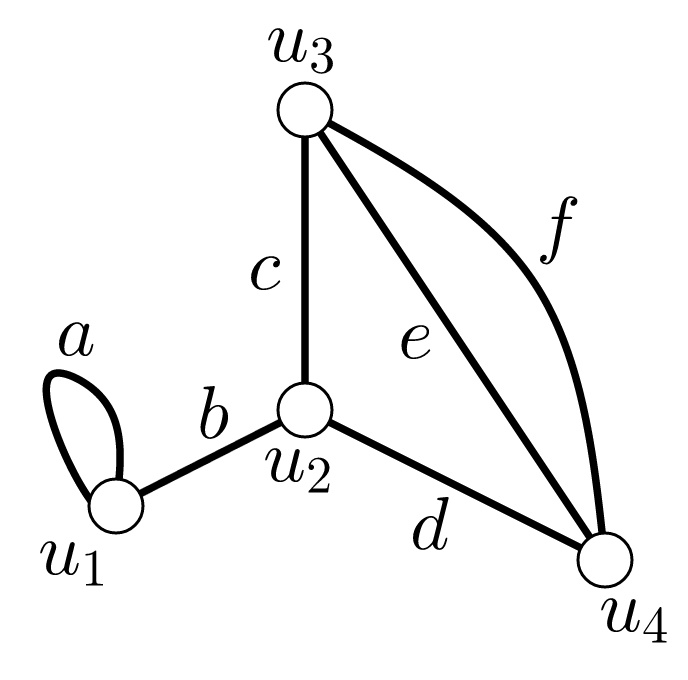
\includegraphics[scale=0.23]{img/imgchapter1/GrafoDefinicion.jpg}
    \caption{}
    \label{fig:diagrama}
\end{figure}

Es común referirse al diagrama como la gráfica en sí. Por tanto, los puntos del diagrama serán llamados también \textit{vértices} y sus líneas \textit{aristas}. La función de incidencia queda ya implícita, pues en el diagrama se muestran las adyacencias entre vértices y aristas.

Para simplificar el discurso (y cuando no haya riesgo de ambigüedad), suele omitirse la letra ``$G$'' de los símbolos que usamos para denotar los conjuntos de vértices y aristas; así, escribimos ``$V$'' en vez de ``$V(G)$'' y ``$E$'' en lugar de ``$E(G)$''. También la función de incidencia queda sobrentendida.

Sea $G$ una gráfica y tomemos $e \in E$. Si sus extremos son iguales, se dice que $e$ es un \textit{lazo}\index{Lazo}. Si hay alguna otra arista, digamos $a$, con los mismos extremos que $e$, entonces decimos que $e$ y $a$ son \textit{aristas paralelas}\index{Arista! paralela}.
\begin{ejem}
En la gráfica de la figura \ref{fig:diagrama}, la arista $a$ es un lazo, pues $u_{1}$ es su único extremo. Mientras que las aristas $e$ y $f$ son paralelas, ya que $u_{3}$ y $u_{4}$ son sus extremos.

\hfill $\blacklozenge$
\end{ejem}
El \textit{grado de un vértice} \index{Grado} es la cantidad total de aristas adyacentes en un vértice dado (los lazos se cuentan doble). A tal número se le denota por $d(v)$, y  $d_{G}(v)$ para enfatizar a qué gráfica pertenece el vértice $v$. Por ejemplo, basándonos en la figura \ref{fig:diagrama}, $d(u_{1})=3$ y $d(u_{4}) = 3$. Una de las propiedades más importantes de los grados es que \textit{la suma total de todos los grados de los vértices de una gráfica es, necesariamente, igual al doble del número de aristas en dicha gráfica}. En la sección \ref{sec:matriz} se dará una justificación de este hecho.

Decimos que $G$ es una \textit{gráfica simple}\index{Gráfica! simple} si no tiene lazos ni aristas paralelas. En tal caso, suele considerarse que $E(G) \subseteq V(G) \times V(G)$ (y la función de incidencia es la \textit{función inclusión de} $E(G)$). 

\subsection{Tipos de gráficas} \label{sec:tiposdegraficas}
Una gráfica es \textit{finita} \index{Gráfica! finita}si sus conjuntos de vértices y aristas son finitos. Todas las gráficas que se estudian en este trabajo son finitas. Si estos conjuntos son vacíos, entonces la gráfica $(\emptyset, \emptyset)$ es \textit{nula}\index{Gráfica! nula}. 

Tomemos $n$ vértices (con $n\geq 1$), digamos $u_{1}, \ldots, u_{n}$ . La \textit{gráfica vacía} es la gráfica $\varnothing := (\{u_{1}, \ldots, u_{n}\}, \emptyset)$, es decir, $\varnothing$ es una gráfica que no tiene aristas. Si se quiere enfatizar el número de vértices de la gráfica vacía, entonces escribimos $\varnothing_{n}$. Si la gráfica consiste de un sólo vértice, decimos que es \textit{trivial}\index{Gráfica! trivial}. Cabe aclarar lo siguiente: cuando hablemos del \textit{conjunto vacío}, lo haremos utilizando el símbolo ``$\emptyset$''; por otro lado, el símbolo ``$\varnothing$'' representa a la gráfica vacía. El conjunto vacío y la gráfica vacía \textit{no} deben ser confundidos.

Decimos que $H$ es \textit{subgráfica} \index{Subgráfica} de $G$ si $V(H) \subseteq V(G)$ y $E(H) \subseteq E(G)$ y $\psi_{H}$ es la \textit{restricción de} $\psi_{G}$ \textit{a} $E(H)$. Si lo anterior sucede, escribimos $H \subseteq G$. Una subgráfica de $G$ es \textit{generadora} \index{Gráfica!generadora} si su conjunto de vértices es exactamente el mismo que $G$, es decir, $H \subseteq G$ es \textit{generadora} si $V(H)=V(G)$.

Sea $X \subseteq V(G)$. La \textit{subgráfica inducida por} \index{Gráfica! inducida} $X$, $G[X]$ es aquella cuyo conjunto de vértices es $X$ y sus aristas son aristas de $G$ que tienen sus extremos en $X$. Similarmente, si $S\subseteq E(G)$, $G[S]$ denota la \textit{subgráfica inducida por} $S$, cuyo conjunto de aristas es $S$ y su conjunto de vértices queda determinado por los extremos de las aristas en $S$. Para evitar confusiones, también decimos que $G[S]$ es una \textit{subgráfica inducida por aristas}. En particular, $G[S]$ es una \textit{subgráfica generadora inducida por aristas} si $S$ es su conjunto de aristas y conserva todos los vértices originales, es decir, su conjunto de vértices es $V(G)$.

Una \textit{gráfica completa} \index{Gráfica! completa}es una gráfica simple en la que cualesquiera dos vértices son adyacentes. Si tal gráfica consta de $n$ vértices, se le escribe como $K_{n}$. En el inciso $(a)$ de la figura \ref{fig:grafoscompletos} mostramos la gráfica completa de $5$ vértices.

Una \textit{gráfica bipartita}\index{Gráfica! bipartita} es una gráfica simple en la que su conjunto de vértices puede partirse en dos conjuntos, digamos $X$ y $Y$, de tal forma que cualquier arista tenga uno de sus extremos en $X$ y el otro en $Y$ (y, por tanto, que no haya aristas que unan dos vértices de $X$, ni tampoco de $Y$). Suele denotarse como $G[X,Y]$. 

Sea $G[X,Y]$ gráfica bipartita y supongamos que en $X$ y $Y$ hay $n$ y $m$ vértices, respectivamente. Si sucediera que todos los vértices de $X$ son adyacentes a todos los de $Y$, entonces decimos que $G[X,Y]$ es una \textit{gráfica bipartita completa}\index{Gráfica! bipartita completa} y se escribe $K_{n,m}$. En el inciso $(b)$ de la figura \ref{fig:grafoscompletos} está la gráfica $K_{3,2}$.

\begin{figure}[h]
    \centering
    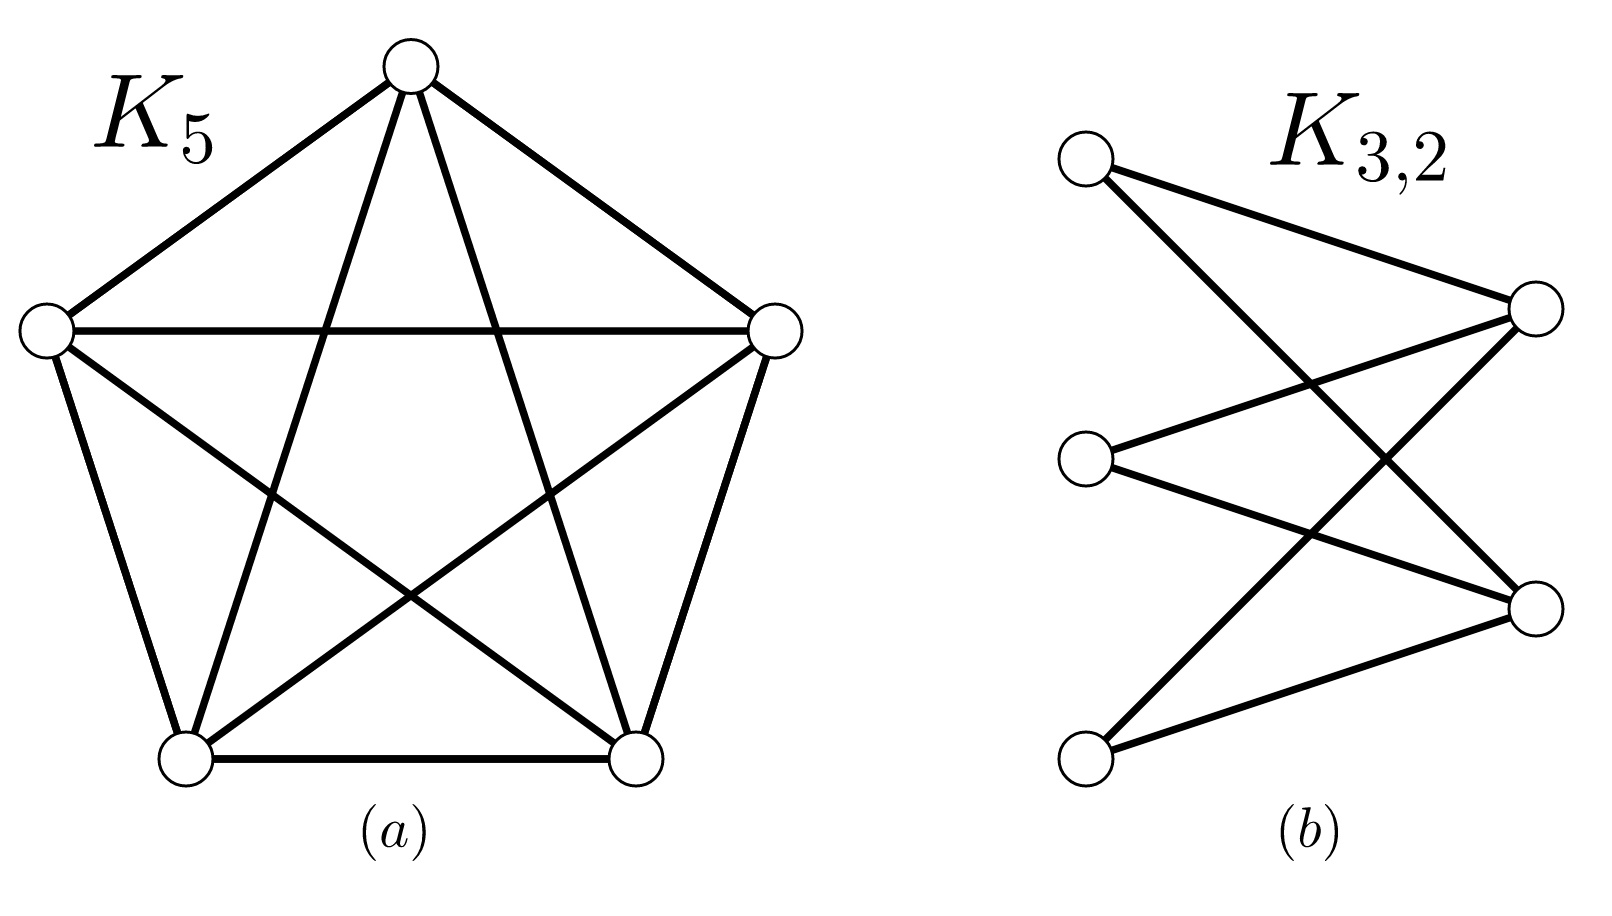
\includegraphics[scale=0.2]{img/imgchapter1/GrafosCompletos.jpg}
    \caption{}
    \label{fig:grafoscompletos}
\end{figure}

Una \textit{gráfica conexa} \index{Gráfica! conexa} es aquella en la que dada cualquier partición $(X,Y)$ de su conjunto de vértices, siempre hay al menos una arista con un extremo en $X$ y otro en $Y$. Si sucediera lo contrario, es decir, que exista una partición de sus vértices en los que no hay aristas entre tales conjuntos, entonces decimos que la gráfica no es conexa o \textit{inconexa}.

La definición clásica de \textit{ciclo}\index{Ciclo} nos dice que es una gráfica conexa en la que todos sus vértices tienen grado $2$. La notación que suele utilizarse es $C_{n}$, donde $n$ es el número de vértices del ciclo; y es fácil notar que también debe tener $n$ aristas. A este número $n$ se le conoce como la \textit{longitud}\index{Longitud! de un ciclo} del ciclo. Así, bajo esta definición, un ciclo de longitud $1$ es, necesariamente, un lazo; y uno de longitud $2$ consta de un par de aristas paralelas. Véase la figura \ref{fig:ciclos}. \textcolor{red}{NO SÉ SI CAMBIAR LA DEFINICIÓN DE CICLO AQUÍ O EN EL CAPÍTULO 2}

\begin{figure}[h]
    \centering
    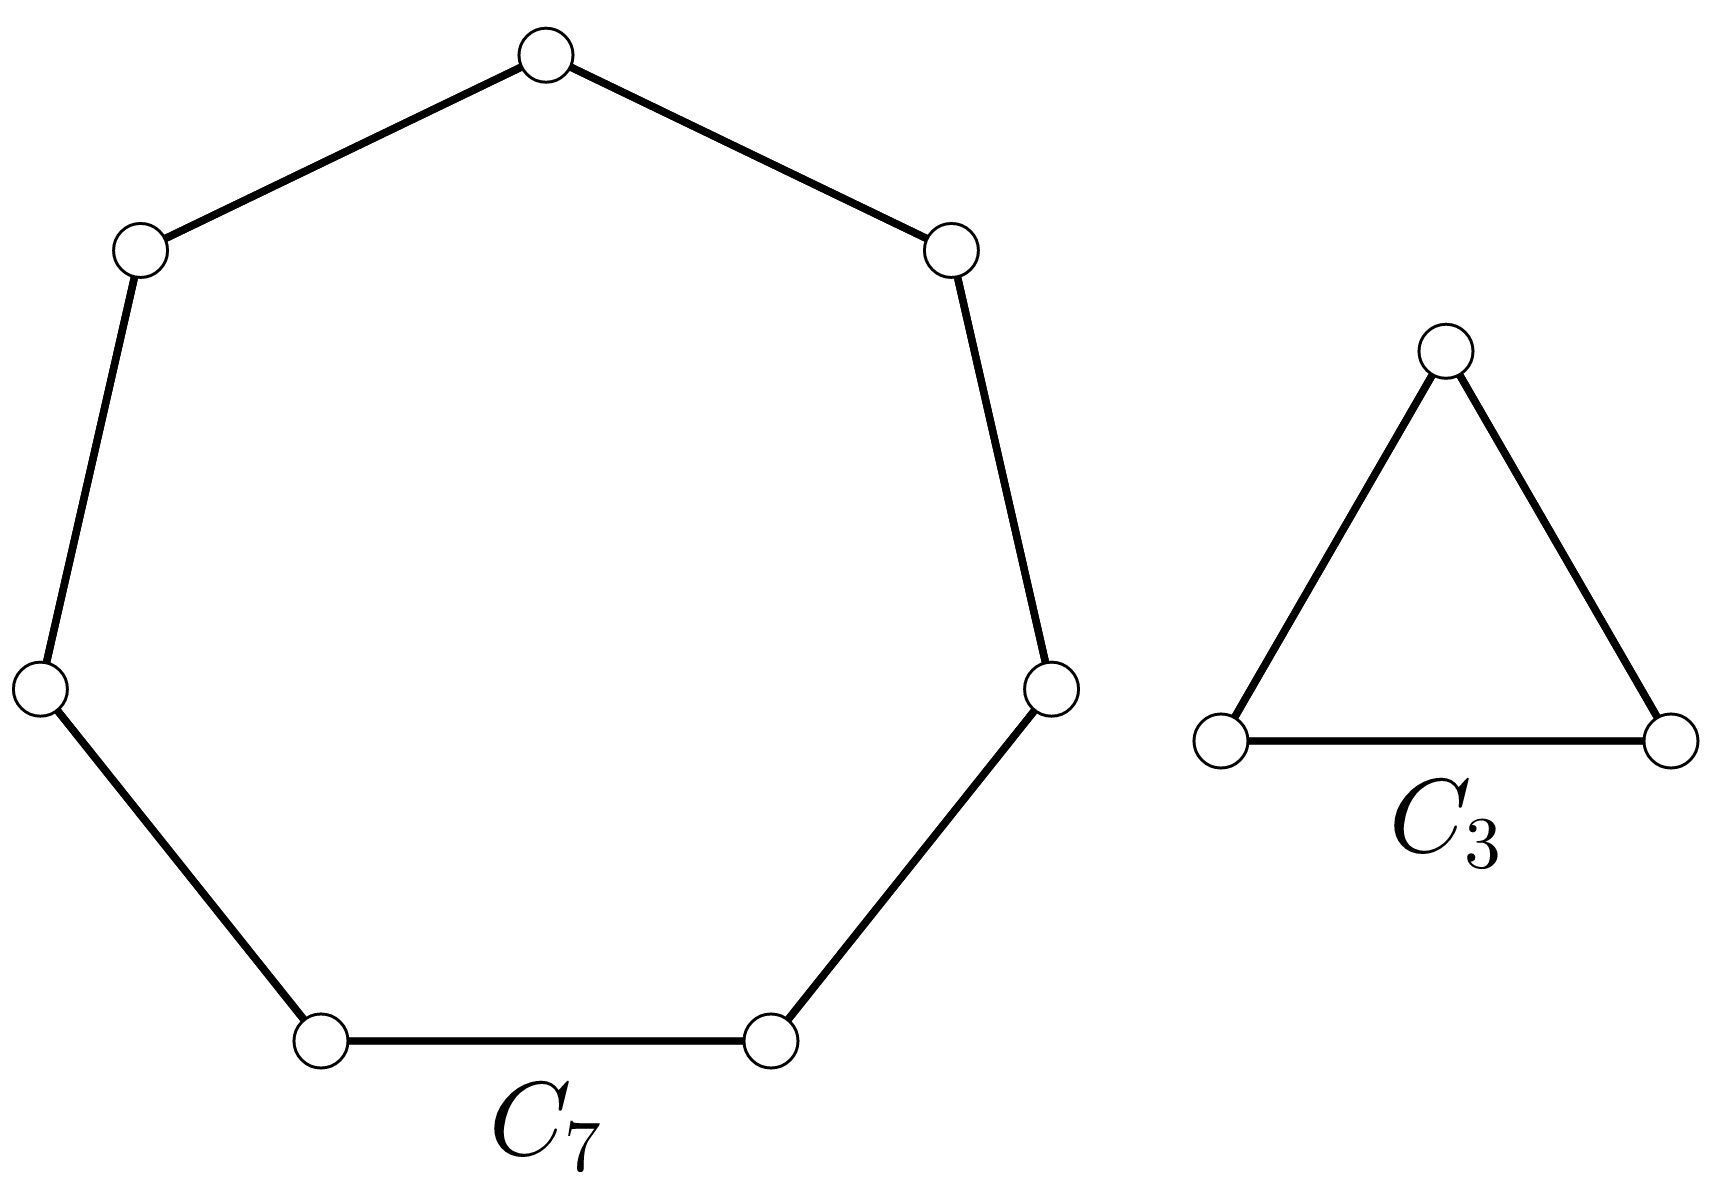
\includegraphics[scale=0.15]{img/imgchapter1/Ciclos.jpg}
    \caption{}
    \label{fig:ciclos}
\end{figure}

%Decimos que $u_{1}, \ldots, u_{n}$ ($n \geq 3$) forman un \textit{ciclo} si $u_{i}$ es %adyacente a $u_{i+1}$, con $i \in \{1, \ldots, n-1 \}$ y $u_{n}$ es adyacente a $u_{1}$. 
Los ciclos y su longitud son bastante útiles para caracterizar ciertas propiedades. Hechos tales como: que \textit{un ciclo es bipartito si y sólo si es de longitud par}; y que \textit{una gráfica es bipartita si y sólo si no contiene ciclos de longitud impar}, son ampliamente usados en la Teoría de Gráficas.

De hecho, el siguiente teorema nos será de mucha ayuda, pues ofrece condiciones necesarias para la existencia de ciclos.

%\renewcommand{\labelenumi}{\textnormal{\alph{enumi})}}
\begin{teo} \label{teo:ciclos}  
Si $G$ es una gráfica en la que todos sus vértices tienen grado al menos dos, entonces $G$ contiene un ciclo.
\end{teo}

\begin{teo}
Si $G$ es una gráfica con $n$ vértices y $m$ aristas, de tal manera que $m \geq n$ (o sea, que hay más aristas que vértices), entonces $G$ contiene un ciclo.
\end{teo}


\subsection{Conexidad} \label{sec:conexidad}
 
Un \textit{camino} \index{Camino} en una gráfica $G$ es una sucesión $W:= u_{0}e_{1}u_{1}\ldots u_{l-1}e_{l}u_{l}$ de vértices y aristas de tal forma que $u_{i-1}$ y $u_{i}$ son extremos de $e_{i}$, con $i\in\{1, \ldots, l\}$. Los vértices y aristas que aparecen en $W$ no son necesariamente distintos.


\begin{ejem} \label{ejem:caminos}
Consideremos la gráfica $G$ con vértices $\{u_{1}, \ldots, u_{5}\}$ y aristas $\{e_{1}, \ldots, e_{7}\}$, como se muestra en la figura \ref{fig:GrafoCaminos}.
Entonces $W_{1}=u_{3}e_{5}u_{4}e_{5}u_{3}e_{3}u_{2}$, $W_{2}=u_{3}e_{4}u_{3}e_{5}u_{4}e_{6}u_{5}$ y $W_{3}=u_{5}e_{7}u_{4}e_{6}u_{5}e_{7}u_{4}e_{5}u_{3}e_{2}u_{1}$ son caminos en $G$. 

\begin{figure}[H]
    \centering
    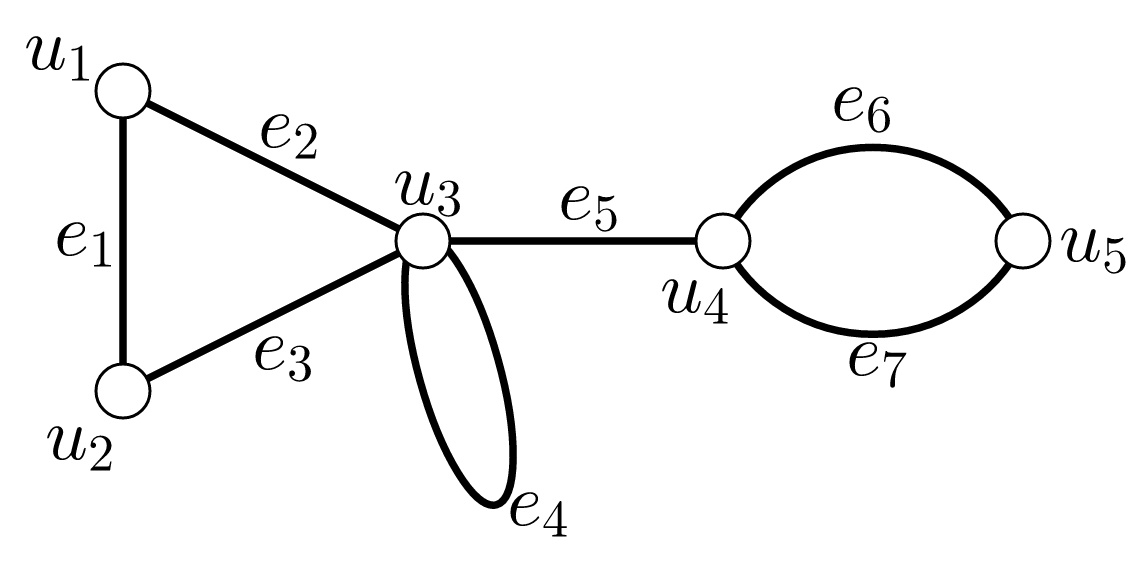
\includegraphics[scale=0.3]{img/imgchapter1/GrafoCaminos.jpg}
    \caption{}
    \label{fig:GrafoCaminos}
\end{figure}

\hfill $\blacklozenge$
\end{ejem}


Si $x = u_{0}$ y $y = u_{l}$, decimos que $W$ es un $xy-camino$ y que $x$ y $y$ son los \textit{extremos}\index{Vértice! extremo} de $W$, los demás son vértices \textit{internos}\index{Vértice! interno}; suele emplearse la notación $xWy$. También se dice que $W$ \textit{conecta} a los vértices $x$ y $y$. Cuando las gráficas sean simples, los caminos se describen en términos de sus vértices, es decir, se omiten las aristas.

La \textit{longitud} \index{Longitud! de un camino} $W$ es la cantidad de aristas empleadas en el camino $W$.

\begin{ejem}
El camino $W_{1}$ del ejemplo \ref{ejem:caminos} es un $u_{3}u_{2}-camino$ y su longitud es igual a $3$ porque utiliza las aristas $e_{5}$ (dos veces) y $e_{3}$.

El camino $W_{2}$ es un $u_{3}u_{5}-camino$ de longitud $3$ y $W_{3}$ es un $u_{5}u_{1}-camino$ de longitud $5$.


\hfill $\blacklozenge$
\end{ejem}


\begin{wrapfigure}{l}{0.35\textwidth}
%\vspace{-1.2cm}
\centering
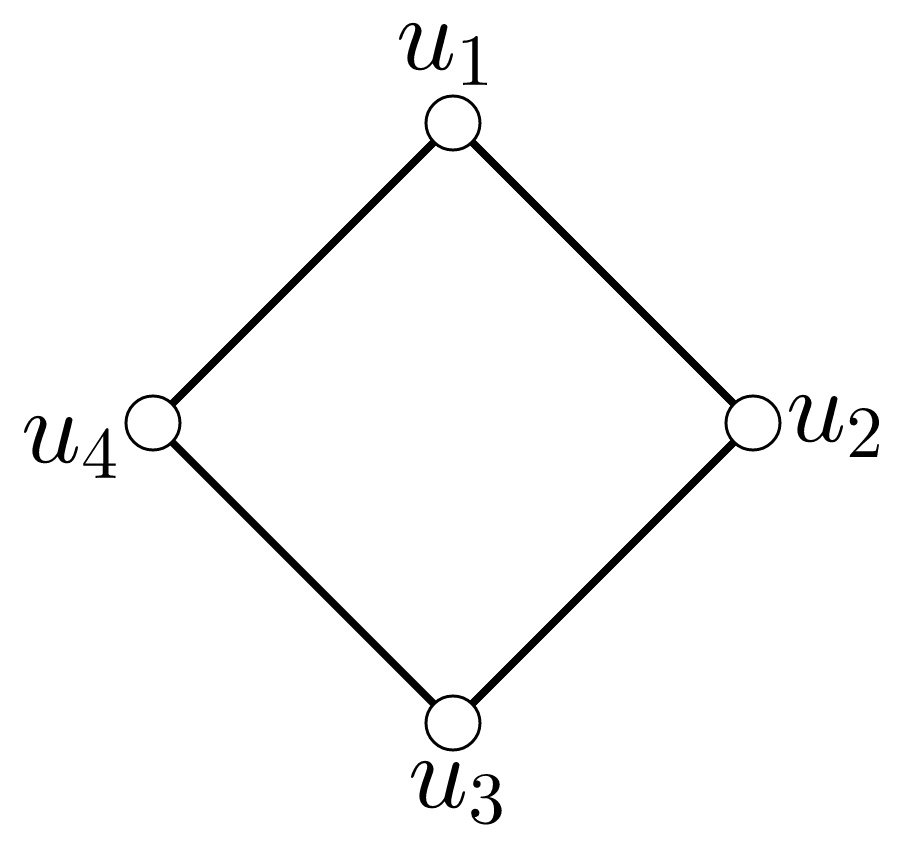
\includegraphics[scale=0.2]{img/imgchapter1/GrafoCiclo.jpg}
\caption{}
\label{fig:cicloc4}
\vspace{-0.5cm}
\end{wrapfigure}
Los caminos se clasifican dependiendo de las características de sus vértices y aristas. En efecto, decimos que un camino es \textit{cerrado} \index{Camino! cerrado} si sus extremos coinciden;si no, es \textit{abierto} \index{Camino! abierto}. Un \textit{paseo} \index{Paseo} es un camino en el que todas sus aristas son distintas; y una \textit{trayectoria} \index{Trayectoria} es un camino en el que todos sus vértices son diferentes (y, por tanto, sus aristas también). 


Un $xy-paseo$ es un paseo cuyos extremos son los vértices $x$ y $y$. Una $xy-trayectoria$ se define análogamente. Además, cuando un paseo es cerrado (i.e., sus extremos son iguales) lo llamamos \textit{circuito} \index{Circuito}. Por último, un circuito en el que todos sus vértices internos son distintos corresponde a los vértices y aristas de un ciclo; de manera inversa, a cada ciclo podemos asignarle un paseo cerrado, aunque no de manera única. Para convencerse de esto, consideremos el ciclo $C_{4}$ de la figura \ref{fig:cicloc4}. Es claro que tanto $\Gamma_{1} = u_{1}u_{2}u_{3}u_{4}$ como $\Gamma_{2} = u_{4}u_{3}u_{2}u_{1}$ son dos circuitos que describen el mismo ciclo $C_{4}$. No obstante, será común que, cuando hablemos de ciclos, lo hagamos considerando alguno de sus circuitos asociados y referirnos a este paseo cerrado como el ciclo en sí. 

\begin{ejem}
Considerando ahora la gráfica \ref{fig:GrafoCaminos2}, es sencillo notar que un camino cerrado es $W_{1}=u_{1}u_{2}u_{6}u_{2}u_{1}$. 
 \begin{figure}[H]
    \centering
    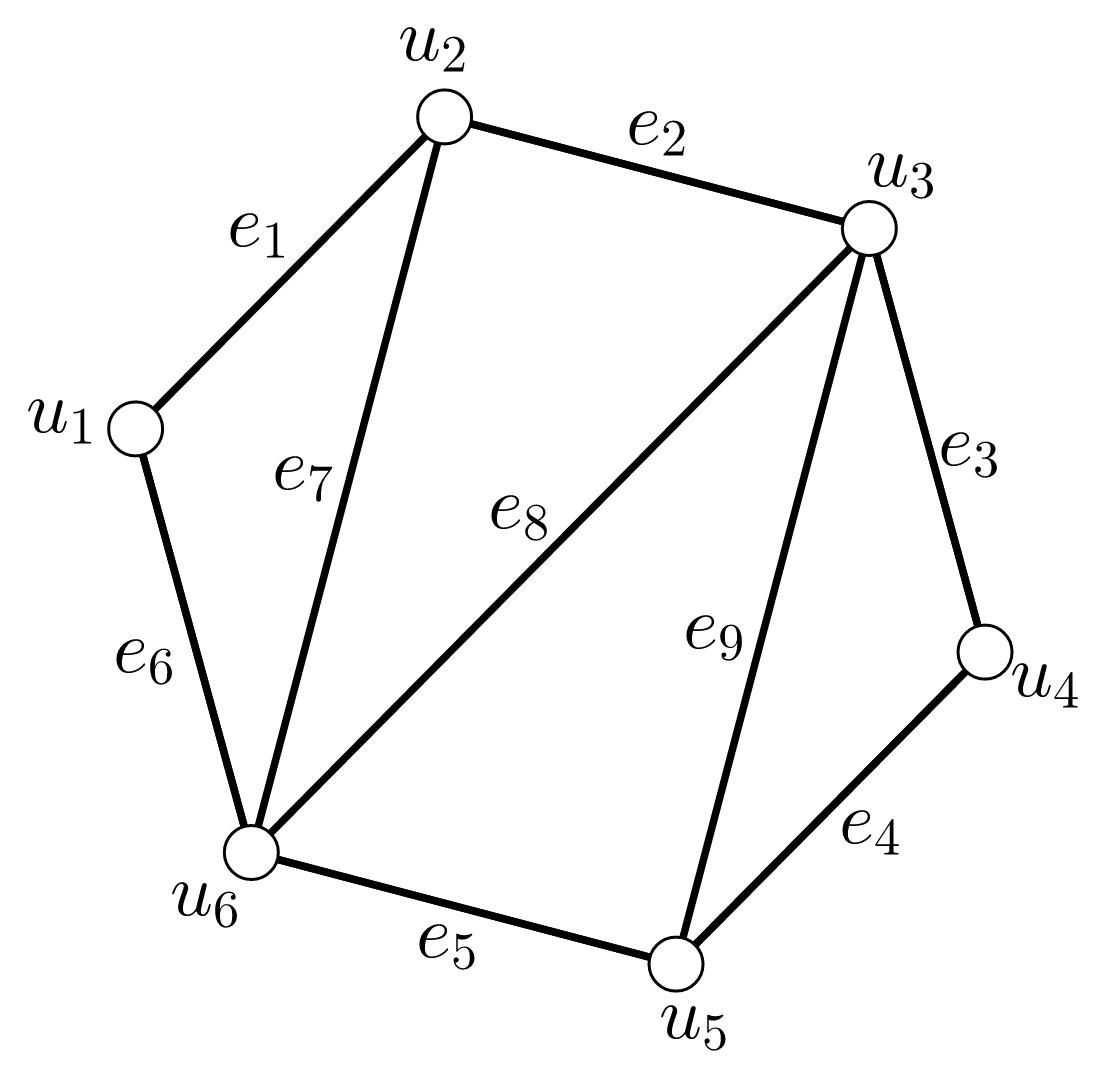
\includegraphics[scale=0.22]{img/imgchapter1/GrafoCaminos2.jpg}
    \caption{}
    \label{fig:GrafoCaminos2}
\end{figure}
Un paseo y una trayectoria serían $W_{2}=u_{5}e_{4}u_{4}e_{3}u_{3}e_{9}u_{5}e_{5}u_{6}e_{7}u_{2}$ y $W_{3} = u_{1}u_{2}u_{3}u_{4}$, respectivamente. Mientras que un circuito es $W_{4}=u_{2}u_{6}u_{3}u_{5}u_{4}u_{3}u_{2}$ y $W_{5}=u_{3}u_{4}u_{5}$ es un ciclo.

\hfill $\blacklozenge$
\end{ejem}

Se sabe bien que \textit{todo $uv-camino$ cerrado contiene un ciclo}. Más aún, \textit{que todo $uv-camino$ contiene una $uv-trayectoria$}. Estos nuevos conceptos nos permiten dar una nueva definición de conexidad, totalmente equivalente a la que dimos al principio. Efectivamente, una gráfica $G$ es \textit{conexa} si y sólo si, para cualquier par de vértices $u$ y $v$, existe una $uv-trayectoria$. Ambas versiones de la definición de conexidad serán usadas indistintamente a lo largo de este trabajo.

\subsection{Operaciones en gráficas}
Hay varias \textit{operaciones} que se pueden realizar entre gráficas. A continuación, se detallan aquellas que más se usaremos en este trabajo.

Dadas dos gráficas $G$ y $H$, su \textit{unión}\index{Unión de gráficas} $G \cup H$ es la gráfica cuyos conjuntos de vértices y aristas son, respectivamente, $V(G) \cup V(H)$ y $E(G) \cup E(H)$. Su \textit{intersección}\index{Intersección de gráficas} $G \cap H$ tiene como vértices y aristas $V(G) \cap V(H)$ y $E(G) \cap E(H)$, respectivamente. La \textit{diferencia simétrica} de $G$ y $H$ está determinada por la diferencia simétrica de sus aristas, i.e., es la gráfica $G \triangle H$ con $V(G) \cup V(H)$ como conjunto de vértices y $E(G)\triangle E(H)$. Véase la figura \ref{fig:operaciones}.

\begin{figure}[H]
    \centering
    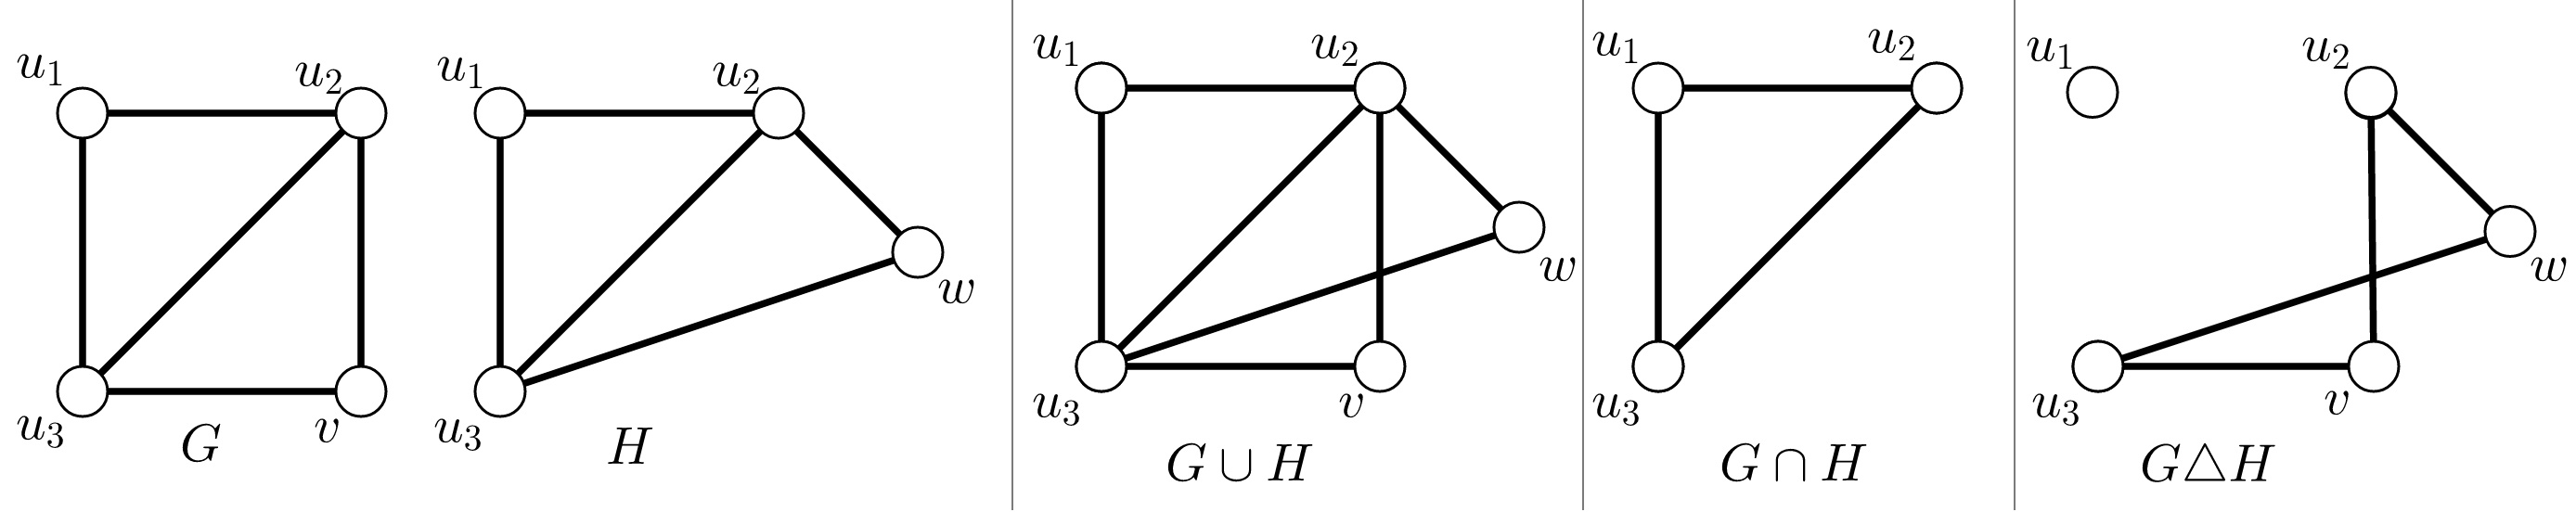
\includegraphics[scale=0.18]{img/imgchapter1/Operaciones.jpg}
    \caption{}
    \label{fig:operaciones}
\end{figure}

Diremos que $G$ y $H$ son \textit{ajenas} \index{Unión de gráficas! ajenas} si no tienen vértices en común; y que son \textit{ajenas por aristas} si tampoco tienen aristas en común. De esta manera, si $G$ y $H$ son ajenas (o ajenas por aristas), decimos que $G \cup H$ es una \textit{unión ajena} (o \textit{ajena por aristas}). 

Si una gráfica es inconexa, entonces puede expresarse como una unión ajena de gráficas conexas, las cuales llamamos \textit{componentes conexas}\index{Componentes conexas}. A la cantidad total de componentes conexas de una gráfica $G$ se le denota por $c(G)$. Si $G$ es conexa, entonces $c(G)=1$.

Si $e \in E(G)$, entonces $G\setminus e$ es la gráfica que resulta de remover la arista $e$ de $G$ (conservando los vértices). Si $S\subseteq E(G)$, $G\setminus S$ se define de manera análoga. Si $e$ es una arista con extremos en $V(G)$ que no pertenece a $E(G)$, la gráfica $G+e$ es aquella que añade $e$ a la gráfica $G$. Similarmente, se define $G + S$, donde $S$ es un conjunto de aristas que no están en $E(G)$ y sus extremos son vértices de $G$.


\subsection{Bosques y árboles} \label{sec:arboles}
\begin{wrapfigure}{r}{0.55\textwidth}
\vspace{-1cm}
 \centering
  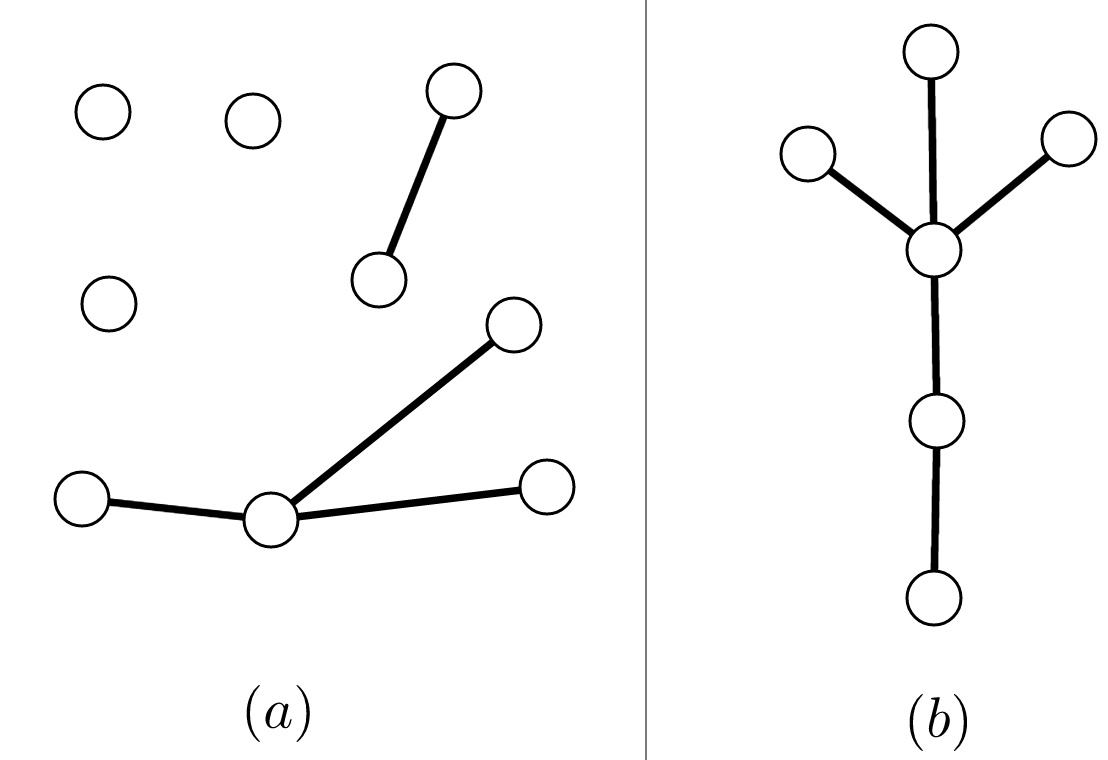
\includegraphics[scale=0.25]{img/imgchapter1/arboles.jpg}
  \caption{}
  \label{fig:arboles}
\end{wrapfigure}
Un \textit{bosque}\index{Bosque} es una gráfica sin ciclos. Si un bosque es conexo, se le dice \textit{árbol} \index{Árbol}. Luego, un árbol es una gráfica conexa sin ciclos. Se desprende de aquí que las componentes conexas de los bosques son, precisamente, árboles. Un  árbol que consta de un sólo vértice es un \textit{árbol trivial}. En caso contrario, es \textit{no trivial}. Desde luego, un \textit{bosque trivial} se compone de árboles triviales. 

Los árboles son la columna vertebral de las gráficas. Su importancia es enorme  debido a sus aplicaciones. Muchísimos resultados provienen de este concepto. De hecho, jugarán un papel clave en esta tesis. En lo que sigue mencionaremos algunas de sus propiedades

\begin{prop}\label{prop:treepath}
Dos vértices cualesquiera en un árbol están conectados por una única trayectoria.
\end{prop}

En virtud de la contrapositiva del teorema \ref{teo:ciclos}, todo bosque tiene un vértice de grado a lo más igual a uno. De hecho, se tiene lo siguiente.

\begin{prop} \label{prop:hojas}
Todo árbol no trivial tiene al menos dos vértices de grado uno. 
\end{prop}

En general, todo bosque no trivial también tendrá al menos dos vértices de grado uno.  

En un bosque son \textit{hojas} los vértices que tienen grado uno. Así, la proposición \ref{prop:hojas} nos garantiza que cualquier árbol no trivial tendrá al menos dos hojas.

La contrapositiva del inciso (b) del teorema \ref{teo:ciclos} asegura que en un bosque hay más vértices que aristas. El teorema que sigue es crucial en el desarrollo de este trabajo. Nos da la cantidad exacta de aristas de un árbol.

\begin{teo} \label{teo:tree}
Si $T$ es cualquier árbol, entonces $|E(T)| = |V(T)|-1$ 
\end{teo}

Suponiendo que $G$ es una gráfica conexa, las subgráficas generadoras de $G$ que son árboles reciben el nombre de \textit{árboles generadores}. De hecho, \textit{cualquier gráfica $G$ es conexa si y sólo si $G$ contiene un árbol generador}.  Por supuesto, si $G$ es inconexa, sus subgráficas generadora acíclicas son \textit{bosques generadores}. Incluso, puede probarse que los bosques generadores maximales son aquellos cuyas componentes conexas son árboles generadores de cada componente conexa de $G$.

Si que $G$ tiene $n$ vértices y suponiendo que es conexa, con base en el teorema \ref{teo:tree}, deducimos que \textit{todo árbol generador de $G$ debe tener $n-1$ aristas}. Luego, si $c:=c(G)$, este hecho se generaliza estableciendo que \textit{todo bosque generador maximal de $G$ consta necesariamente de $n-c$ aristas}. Tales cantidades serán relevantes más adelante.


\subsection{Matriz de incidencia de una gráfica} \label{sec:matriz}
Sea $G$ una gráfica cualquiera con $n$ vértices y $m$ aristas. La \textit{matriz de incidencia de} $G$ \index{Matriz! de incidencia de una gráfica}es la matriz $\mathbf{M}_{G} := [m_{ve}] \in \mathbb{M}_{n \times m}(\mathbb{R})$, donde

$$ m_{ve}=
\begin{cases}
0, & \text{si el vértice } v \text{ no es adyacente a la arista } e \\ 
1, & \text{si } v \text{ es adyacente a } e\\ 
2, & \text{si } e \text{ es un lazo en } v
\end{cases}
$$

En la figura \ref{fig:matrizdeincidencia} mostramos una gráfica y su matriz de incidencia.

\begin{figure}[H]
    \centering
    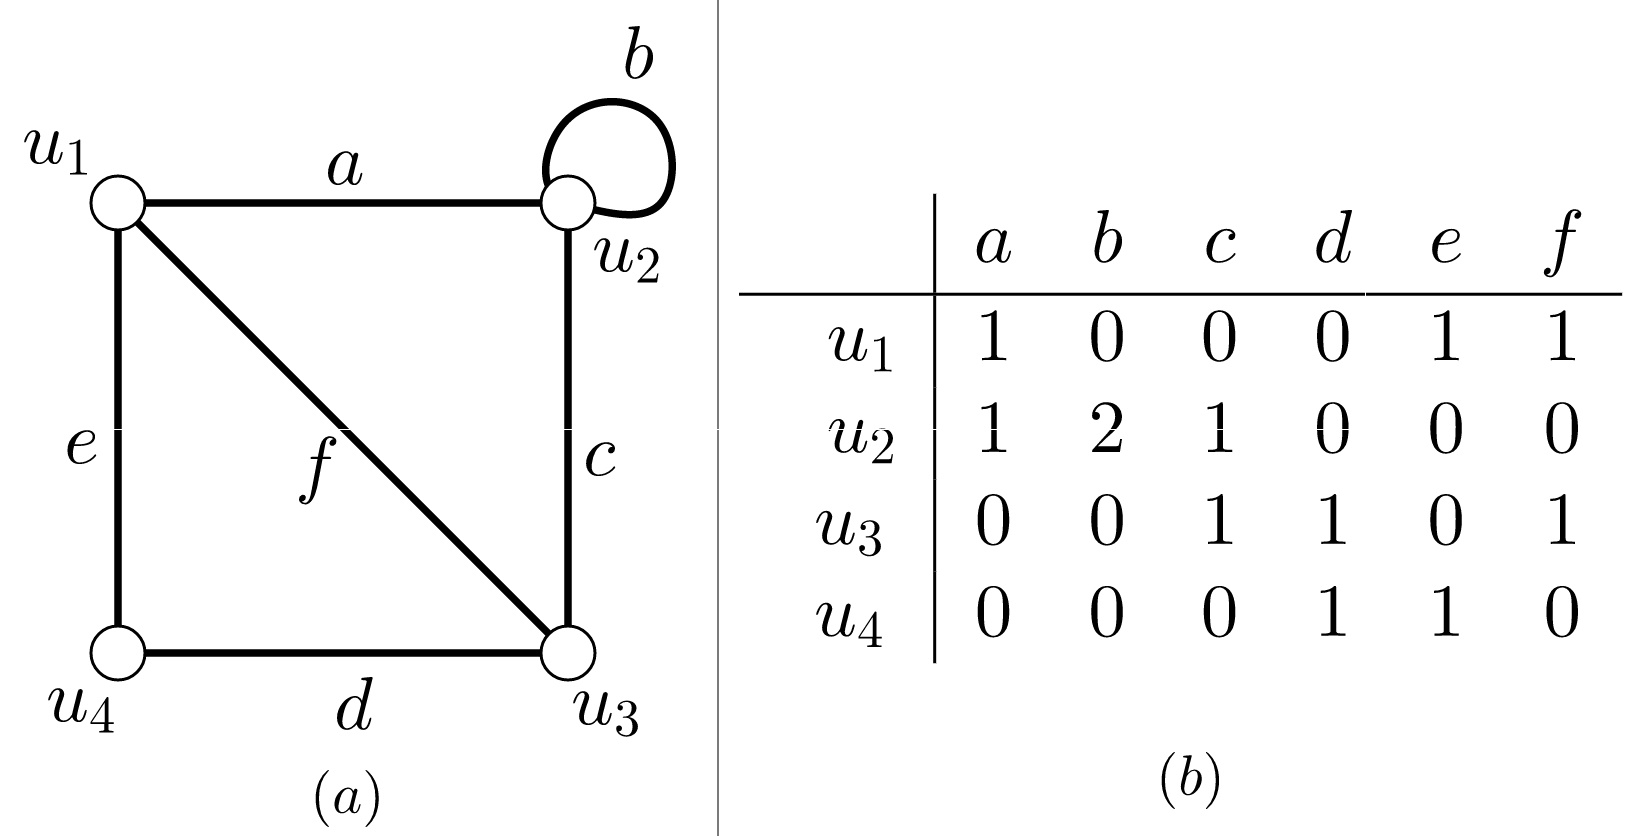
\includegraphics[scale=0.25]{img/imgchapter1/matrizdeincidencia.jpg}
    \caption{}
    \label{fig:matrizdeincidencia}
\end{figure}

Supongamos que $G$ es inconexa y digamos que sus componentes conexas son $F_{1}, \ldots, F_{k}$, dado que los vértices entre diferentes componentes no son adyacentes, se tiene que la matriz de incidencia de $G$ es una matriz diagonal por bloques, donde cada bloque corresponde a la matriz de incidencia de cada componente (siempre y cuando los vértices y las aristas estén etiquetados de manera adecuada):

$$
\mathbf{M}_{G}=\begin{bmatrix}
\mathbf{M}_{F_{1}} & \cdots  & \mathbf{O}\\ 
\vdots & \ddots & \vdots\\ 
\mathbf{O} & \cdots & \mathbf{M}_{F_{k}}
\end{bmatrix}.
$$

Entonces $\mathbf{M}_{G}$ es una matriz que tiene tantos renglones como vértices hay en $G$, y tantas columnas como aristas. Cada una de sus entradas indica qué ``tipo'' de adyacencia hay entre el vértice (renglón) y la arista (columna) correspondientes.  

De lo anterior, es sencillo observar que si tomamos cualquiera de sus renglones, la suma de todas sus entradas es igual al grado del vértice correspondiente, en otras palabras, que $\sum_{e \in E(G)}m_{ve} = d(v)$, con $v$ un vértice fijo.

De igual modo, considerando una columna cualquiera, la suma de todos sus renglones es $2$, pues la arista correspondiente es adyacente a lo más en dos vértices (recordemos que si la arista es un lazo, es adyacente a un único vértice cuyo grado sería $2$). Luego, $\sum_{v \in V(G)}m_{ve} = 2$, con $e$ una arista fija.

La demostración del siguiente teorema (que se mencionó antes) es un primer vistazo de la utilidad y del potencial de la matriz de incidencia para representar y estudiar propiedades de las gráficas desde otros puntos de vista. En los capítulos siguientes desarrollaremos estas ideas.


\begin{teo}
En cualquier gráfica $G$, se cumple que

$$
\sum_{v \in V(G)} d(v) = 2 |E(G)|. 
$$
\end{teo}

\begin{proof}
Es un hecho conocido que la suma total de todas las entradas de una matriz puede obtenerse de dos formas: sumando las entradas columna por columna, o bien sumando las entras renglón por renglón. Esto, respecto a la matriz de incidencia, se traduce en la siguiente igualdad:

$$
\sum_{v \in V(G)} (\sum_{e \in E(G)} m_{ve}) = \sum_{e \in E(G)} (\sum_{v \in V(G)} m_{ve}).
$$
Considerando lo dicho en párrafos anteriores:

$$
\sum_{v \in V(G)} d(v) = \sum_{e \in E(G)} 2.
$$

Así, concluimos que la suma de los grados de todos los vértices de $G$ es igual al doble de sus aristas, o sea, $\sum_{v \in V(G)} d(v) = 2 |E(G)|$.

\end{proof}

\subsection{Digráficas} \label{sec:queesunadigrafica}

Una \textit{gráfica dirigida} \index{Gráfica! dirigida} $D$ (también llamada \textit{digráfica} \index{Digráfica}) es un par ordenado $(V(D), A(D))$, donde $V(D)$ es el conjunto de \textit{vértices}\index{Vértice! de una digráfica} de $D$, y $A(D)$ (ajeno con $V(D)$) su conjunto de \textit{arcos}\index{Arco de una digráfica}; junto con una \textit{función de incidencia} \index{Función de incidencia! de una digráfica}
 $\psi_D \colon A(D) \rightarrow V(D) \times V(D)$ que asigna a cada arco de la digráfica un par ordenado de vértices (no necesariamente diferentes).
 
 Tomando un arco $a$ cualquiera, y suponiendo que $\psi_D (a) = (u,v)$, diremos que $u$ y $v$ son extremos del arco $a$ y que éste \textit{une} a $u$ con $v$ o, mejor dicho, que $u$ \textit{domina} a $v$. También decimos que $u$ es la \textit{cola} \index{Vértice! cola} de $a$ y $v$ su \textit{cabeza \index{Vértice! cabeza}}, y escribimos $t(a) = u$ y $h(a)=v$, respectivamente.
 
 Igual que en las gráficas, solemos representar las digráficas con diagramas \index{Diagrama! de una digráfica} y pensar que éstos son las digráficas en sí. También omitir la función de incidencia y no escribir la letra ``$D$'' de los símbolos que representan los conjuntos de vértices y arcos.
 
 El \textit{ingrado}\index{Ingrado} de $v$, $d_{D}^{-}(v)$, es la cantidad de arcos cuya cabeza es $v$. Similarmente, a la cantidad de arcos cuya cola es $v$ es el \textit{exgrado}\index{Exgrado} de $v$, escrito como $d_{D}^{+}(v)$. El \textit{grado}\index{Grado} de $v$ es sencillamente la suma de su exgrado y su ingrado, i.e., $d_{D}(v) : = d_{D}^{+}(v) + d_{D}^{-}(v)$. Un \textit{pozo} es un vértice de exgrado igual a cero y una \textit{fuente} uno de ingrado igual a cero.
 
 \begin{ejem} \label{ejem:diagramadigrafica}
 Consideremos la digráfica $D = (V(D),A(D))$, con $V(D)=\{u_{1}, u_{2},u_{3},u_{4}\}$ y $E(G)=\{a,b,c,d,e,f,g\}$ y $\psi_{D}$ definida como sigue:

\begin{center}
\begin{tabular}{ c c c c }
$\psi_{D}(a) = (u_{2},u_{1})$& $\psi_{D}(b) = (u_{1},u_{2})$ & $\psi_{D}(c) = (u_{2},u_{3})$ & $\psi_{D}(d) = (u_{3},u_{4})$  \\
$\psi_{D}(e) = (u_{1},u_{4})$  & $\psi_{D}(f) = (u_{1},u_{5})$ & $\psi_{D}(g) = (u_{5},u_{5})$
\end{tabular}
\end{center}

El diagrama que representa a $D$ se muestra en la figura \ref{fig:digraficadiagrama}. En particular, el ingrado de $u_{1}$ es igual a $1$ y su exgrado es $3$. Obsérvese que $u_{4}$ es un pozo pues $d^{+}(u_{4})=0$ y $d^{-}(u_{4})=2$. Nótese además que la cola del arco $d$ es $u_{3}$ y su cabeza es $u_{4}$. De igual modo, $t(f) = u_{1}$ y $h(f)=u_{5}$.
\begin{figure}
    \centering
    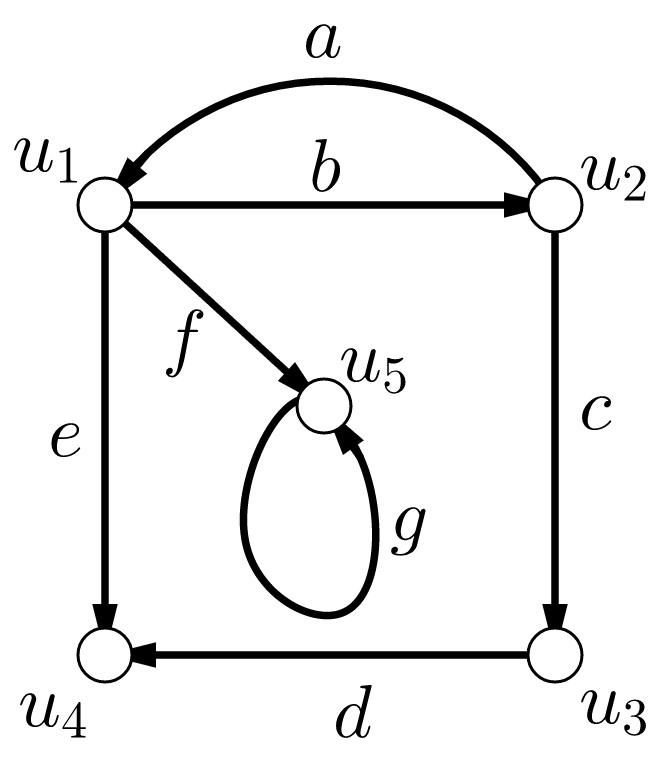
\includegraphics[scale=0.3]{img/imgchapter1/digrafica.jpg}
    \caption{Diagrama de una digráfica}
    \label{fig:digraficadiagrama}
\end{figure}

\hfill $\blacklozenge$
 \end{ejem}
 %De igual modo, tomando $v$ en $V(D)$, se le llama \textit{invecino} a cualquier vértice %que domina a $v$; y \textit{exvecino} a cualquier vértice dominado por $v$. Escribimos %$N_D^{-} (v)$ al conjunto de invecinos de $v$, y $N_D^{+} (v)$ a su conjunto de %exvecinos.
 
 
\subsection{Algunas digráficas, conexidad y matriz de incidencia}
 A partir de una digráfica $D$ cualquiera, podemos obtener la \textit{gráfica subyacente de} $D$, denotada como $G(D)$. Tal gráfica se obtiene de reemplazar los arcos de $D$ por aristas con los mismos extremos. En la figura \ref{fig:subyacente} se muestra la gráfica subyacente de la digráfica del ejemplo \ref{ejem:diagramadigrafica}. Y si invertimos las orientaciones de sus arcos, obtendremos una nueva digráfica llamada su \textit{converso}.
 \begin{figure}[h]
 \centering
    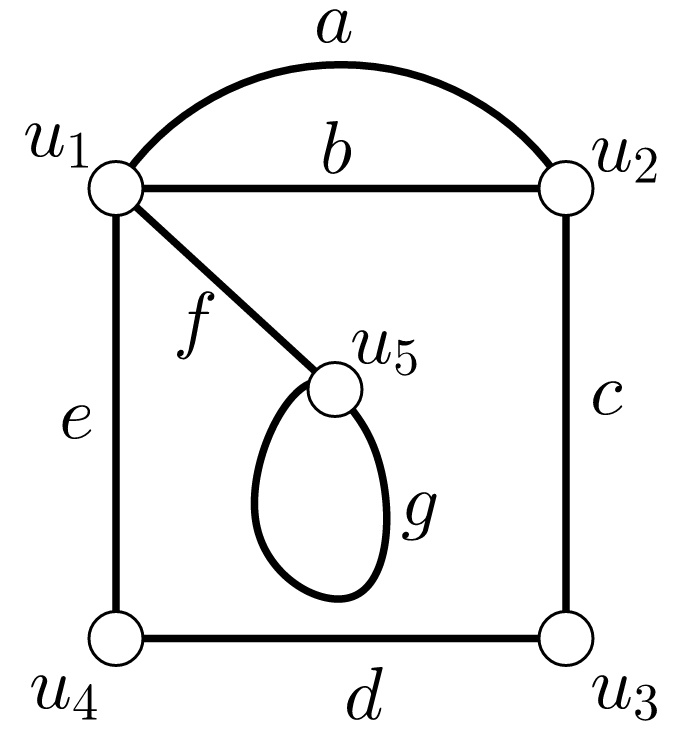
\includegraphics[scale=0.3]{img/imgchapter1/graficasubyacente.jpg}
    \caption{}
    \label{fig:subyacente}
 \end{figure} 
Por otra parte, de una gráfica $G$ es posible construir una digráfica ``orientando'' sus aristas, i.e., reemplazando cada arista por uno de los dos posibles arcos entre sus extremos. Tal digráfica se le conoce como una \textit{orientación de} $G$, y la escribimos $\overrightarrow{G}$. Debe notarse que una gráfica puede tener varias orientaciones.


Muchos de los conceptos en digráficas son similares a los de las gráficas no dirigidas. Por ejemplo, la definición de  \textit{subdigráfica} de un digráfica es análogo a del \textit{subgráfica}. Los ciclos, bosques y árboles de una digráfica son los mismos de su gráfica subyacente (pero conservando las orientaciones de los arcos). Véase la figura \ref{fig:ciclosdigrafica}. 

 \begin{figure}[h]
    \centering
    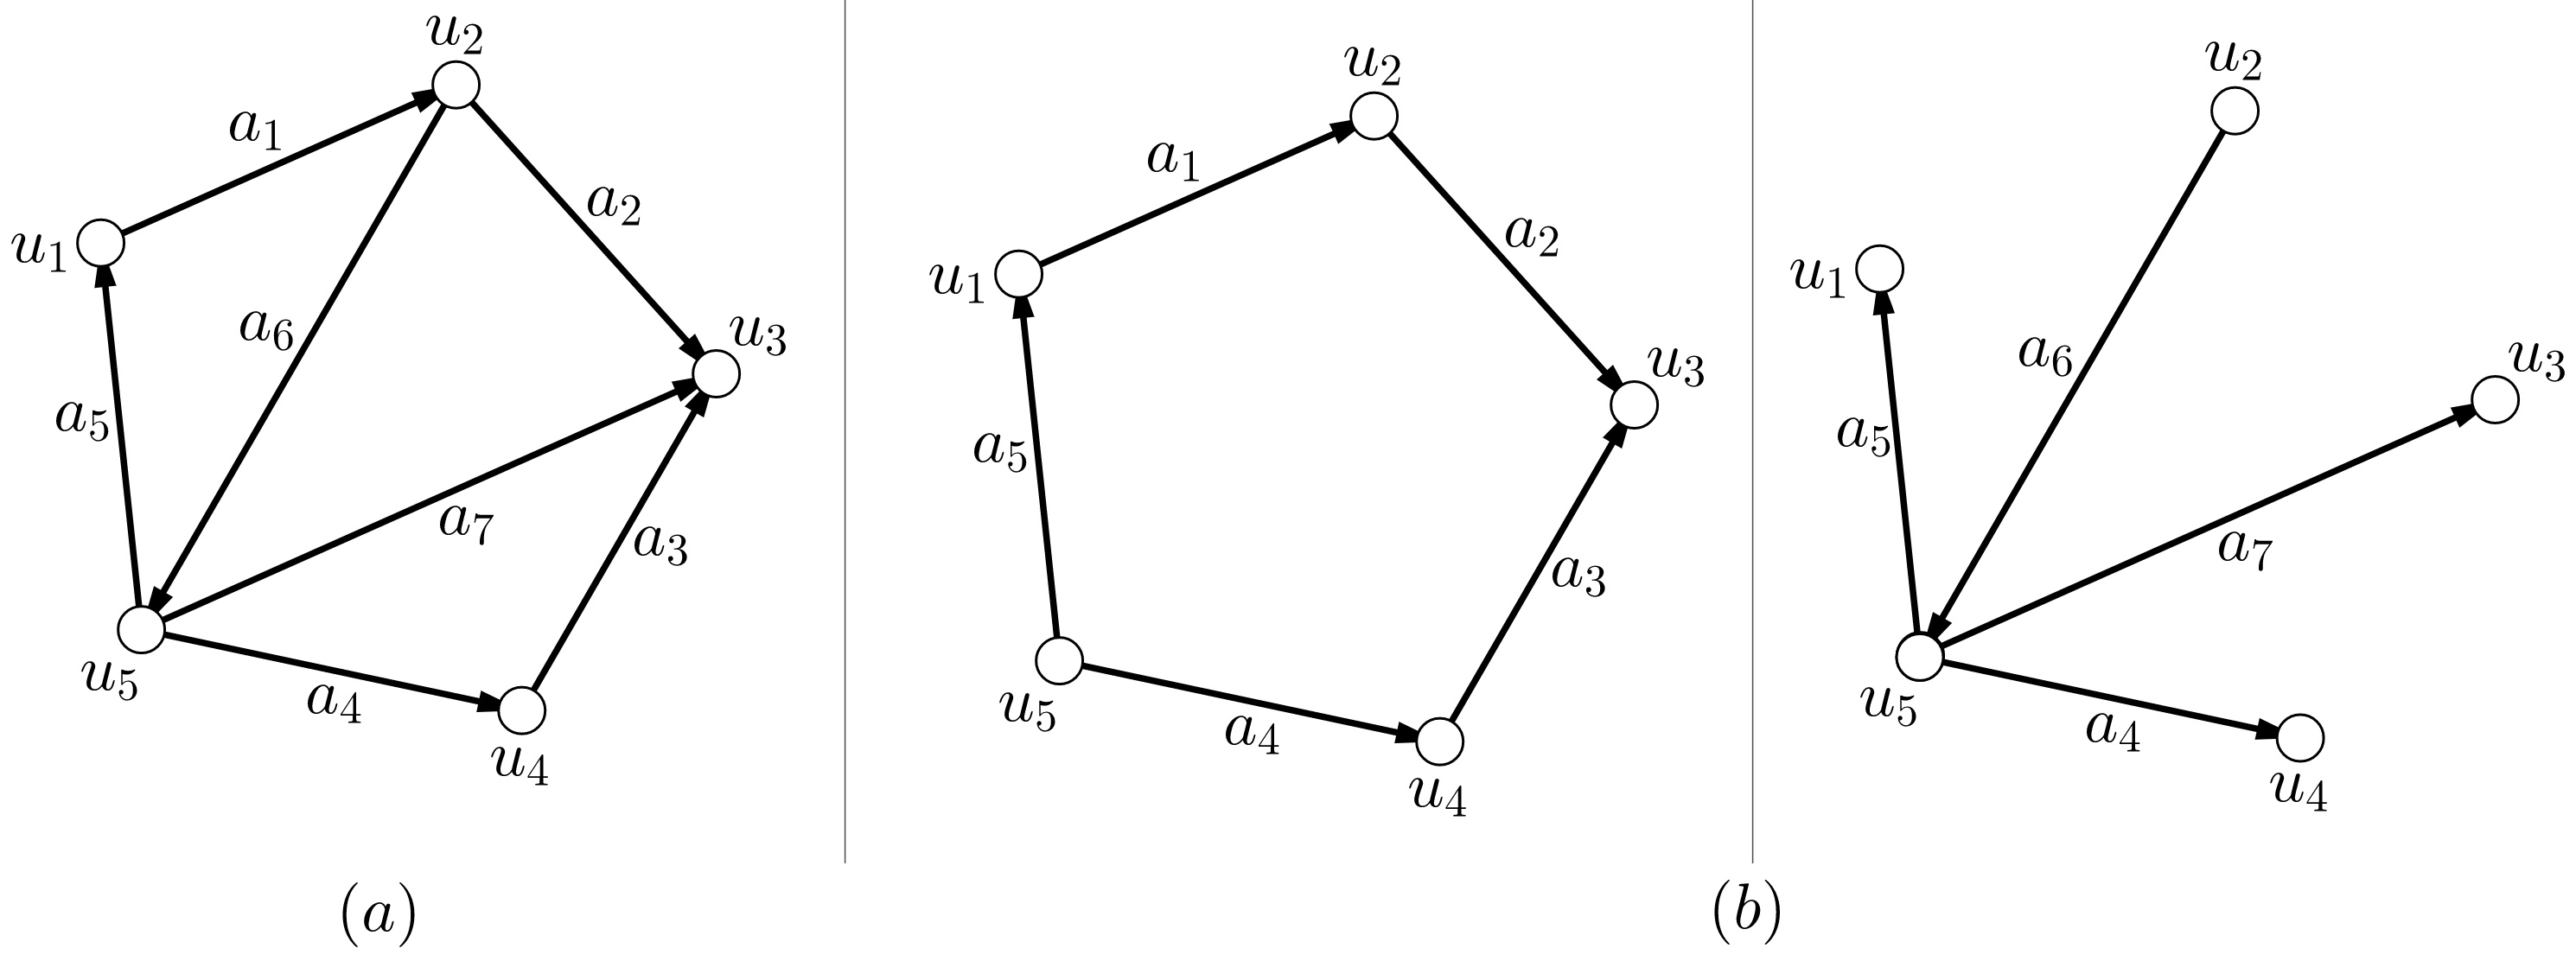
\includegraphics[scale=0.16]{img/imgchapter1/ciclosdigrafica.jpg}
    \caption{Ciclos y árboles en digráficas}
    \label{fig:ciclosdigrafica}
\end{figure}

Un \textit{camino} en una digráfica se define similarmente como en las gráficas: es una sucesión $W:= u_{0}a_{1}u_{1}\ldots u_{l-1}a_{l}u_{l}$ de vértices y arcos de tal forma que $u_{i-1}$ y $u_{i}$ son extremos de $a_{i}$, con $i\in\{1, \ldots, l\}$. Sin embargo, hay que destacar que $u_{i-1}$ no necesariamente domina a $u_{i}$; si fuera el caso, se dice que el camino es \textit{dirigido}. La misma terminología para los caminos en gráficas se usa aquí y las trayectorias, paseos y circuitos también de definen parecido. Retomando la digráfica de la figura \ref{fig:digraficadiagrama}, $W_{1} = u_{1}eu_{4}du_{3}cu_{2}$ y $W_{2}=u_{1}bu_{2}cu_{3}du_{4}$ son caminos y $W_{3}= u_{1}bu_{2}au_{1}fu_{5}gu_{5}$ es un camino dirigido.

Una digráfica es \textit{conexa} si su gráfica subyacente es conexa, y es \textit{fuertemente conexa} si, para cualquier par de vértices $x$ y $y$, existen un $xy-camino$ y un $yx-camino$.  

Las gráficas dirigidas también tienen sus propias matrices de incidencia (véase la figura \ref{fig:matrizdeincidenciadigrafica}). Suponiendo que $D$ una digráfica cualquiera con $n$ vértices y $m$ arcos, su \textit{matriz de incidencia de} es la matriz $\mathbf{M}_{D}:= [m_{va}] \in \mathbb{M}_{n \times m}(\mathbb{R})$, donde
$$ m_{va}=
\begin{cases}
\hspace{0.7em} 1, & \text{si el vértice } v \text{ es cola de } a \text{ y } a \text{ no es un lazo}\\ 
-1, & \text{si } v \text{ cabeza de } a \text{ y } a \text{ no es un lazo}\\ 
\hspace{0.7em} 0, & \text{en otro caso}
\end{cases}
$$

\begin{figure}[h]
    \centering
    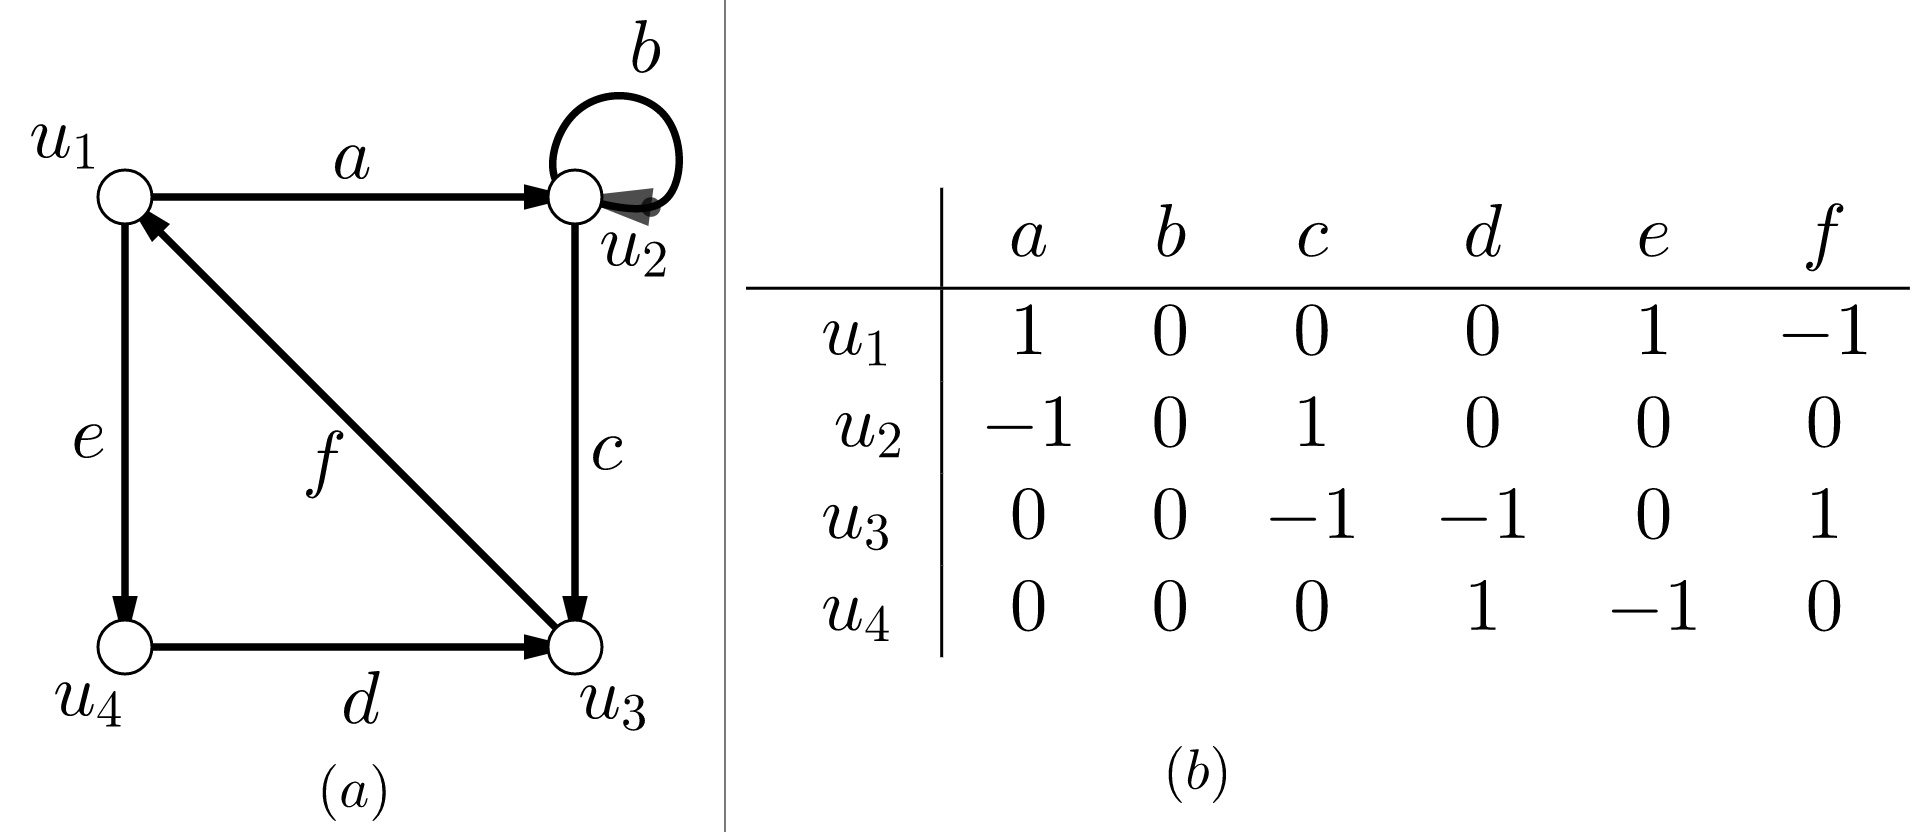
\includegraphics[scale=0.23]{img/imgchapter1/matrizdeincidenciadigrafica.jpg}
    \caption{}
    \label{fig:matrizdeincidenciadigrafica}
\end{figure}

Como es de esperarse, las matrices de incidencia de digráficas inconexas son parecidas a las de las gráficas inconexas, siempre y cuando los vértices y arcos estén etiquetados de manera correcta.






 